%
% Report -- Verilog-A implementation of the EKV v2.6 long and short channel MOSFET models
%
% Copyright (C) 2008 Mike Brinson <mbrin72043@yahoo.co.uk>
%
% Permission is granted to copy, distribute and/or modify this document
% under the terms of the GNU Free Documentation License, Version 1.1
% or any later version published by the Free Software Foundation.
%

% redefine subfigure caption
\renewcommand{\thesubfigure}{\thefigure(\alph{subfigure})}
\makeatletter
  \renewcommand{\@thesubfigure}{\thesubfigure:\space}
  \renewcommand{\p@subfigure}{}
\makeatother

% redefine subtable caption
\renewcommand{\thesubtable}{\thetable(\alph{subtable})}
\makeatletter
  \renewcommand{\@thesubtable}{\thesubtable:\space}
  \renewcommand{\p@subtable}{}
\makeatother

\tutsection{Introduction}

This report presents the background to the Qucs implementation of the
EKV 2.6 long and short channel MOSFET models. During 2007 the Qucs
development team employed the EKV v2.6 MOSFET model as a test case
while developing the Qucs non-linear equation defined devices
(EDD)\footnote{An example EDD macromodel of the short channel EKV 2.6
model can be found at \url{ http://qucs.sourceforge.net/}.}. More
recently complete implementations of the long and short channel EKV
v2.6 models have been developed using the Qucs Verilog-A compact
device modelling route.  This work forms part of the Verilog-A compact
device modelling standardisation initiative\footnote{Stefan Jahn, Mike
Brinson, Michael Margraf, H\'{e}l\`{e}ne Parruitte, Bertrand Ardouin,
Paolo Nenzi and Laurent Lemaitre, GNU Simulators Supporting Verilog-A
Compact Model Standardization, MOS-AK Meeting, Premstaetten, 2007,
\url{http://www.mos-ak.org/premstaetten/papers/MOS-AK_QUCS_ngspice_ADMS.pdf}
}.  The EKV v2.6 MOSFET model is a physics based model which has been
placed in the public domain by its developers. It is ideal for
analogue circuit simulation of submicron CMOS circuits.  Since the
models introduction and development between 1997 and 1999 it has been
widely used in industry and by academic circuit design groups. Today
the EKV v2.6 model is available with most of the major commercial
simulators and a growing number of GPL simulators. The Verilog-A code
for the Qucs ADMS\footnote{Lemaitre L.  and GU B., ADMS - a fully
customizable Verilog-AMS compiler approach, MOS-AK Meeting,
Montreux. Available from
\url{http://www.mos-ak.org/montreux/posters/17_Lemaitre_MOS-AK06.pdf }
} compiled version of the EKV v2.6 model is given in an appendix to
this report.



\tutsection{Effects modelled} 
The EKV v2.6 MOSFET model includes the following effects:
\begin{itemize}
 \item Basic geometrical and process related features dependent on oxide thickness, junction depth, effective channel length and width
 \item Effects of doping profile
 \item Modelling of weak, moderate and strong inversion behaviour
 \item Modelling of mobility effects due to vertical and lateral fields, velocity saturation
 \item Short channel effects including channel-length modulation, source and drain charge-sharing and reverse channel effect
 \item Modelling of substrate current due to impact ionization
 \item Thermal and flicker noise
 \item First order non-quasistatic model for the transconductances
 \item Short-distance geometry and bias dependent device matching
\end{itemize}

The Qucs implementation of the short channel EKV v2.6 model includes
nearly all the features listed above\footnote{This first release of
the Qucs implementation of the EKV v2.6 MOSFET model does not include
the first-order non-quasistatic model for transconductances.}. A
simpler long channel version of the model is also available for those
simulations that do not require short channel effects.  Both nMOS and
pMOS devices have been implemented. No attempt is made in this report
to describe the physics of the EKV v2.6 model. Readers who are
interested in learning more about the background to the model, its
physics and function should consult the following references:

\begin{itemize}
 \item Matthias Bucher \textit{et. al.}, The EPFL-EKV MOSFET Model Equations for Simulation, Electronics Laboratories, Swiss Federal Institute of Technology (EPFL), Lausanne, Switzerland, Model Version 2.6, Revision II, July 1998.
 \item W\l adys\l aw Grabi\'{n}ski \textit{et. al}. Advanced compact modelling of the deep submicron technologies, Journal of Telecommunications and Information Technology, 3-4/2000, pp. 31-42. 
 \item Matthias Bucher \textit{et. al.}, A MOS transistor model for mixed analog-digital circuit design and simulation, pp. 49-96, Design of systems on a chip - Devices and Components, KLUWER Academic Publishers, 2004.
\item Trond Ytterdal \textit{et. al.}, Chapter 7: The EKV model, pp. 209-220, Device Modeling for Analog and RF CMOS Circuit Design, John Wiley $\&$ Sons, Ltd, 2003.
\item Patrick Mawet, Low-power circuits and beyond: a designer's perspective on the EKV model and its usage, MOS-AK meeting, Montreux, 2006, \url{http://www.mos-ak.org/montreux/posters/09_Mawet_MOS-AK06.pdf}
\item Christian C. Enz and Eric A. Vittoz, Charge-based MOS transistor Modeling - The EKV model for low-power and RF IC design, John Wiley $\&$ Sons, Ltd, 2006.
\end{itemize}
 



\tutsection{The Qucs long channel EKV v2.6 model}

A basic DC model for the long channel nMOS EKV v2.6 model is given at
the EKV Compact MOSFET model website\footnote{See
\url{http://legwww.epfl.ch/ekv/verilog-a/} for the Verilog-A
code.}. Unfortunately, this model is only of limited practical use due
to its restricted modelling features\footnote{No dynamic, noise or
temperature effects.}.  It does however, provide a very good
introduction to compact device modelling using the Verilog-A hardware
description language. Readers who are unfamiliar with the Verilog-A
hardware description language should consult the following references:

\begin{itemize}
 \item Accellera, Verilog-AMS Language Reference Manual, Version 2.2, 2004, Available from \url{http://www.accellera.org}.
 \item Kenneth S. Kundert and Olaf Zinke, The Designer's Guide to Verilog-AMS, Kluwer Academic Publishers, 2004.
 \item Dan Fitzpatrick and Ira Miller, Analog Behavioral Modeling with the Verilog-A Language, Kluwer Academic Publishers, 1998.
\item Coram G. J., How to (and how not to) write a compact model in Verilog-A, 2004, IEEE International Behavioural modeling and Simulation Conference (BMAS2004), pp. 97-106.
\end{itemize}

The equivalent circuit of the Qucs EKV long channel n type MOSFET
model is shown in Fig.~\ref{fig:EKV1}.  In this model the inner
section, enclosed with the red dotted box, represents the fundamental
intrinsic EKV v2.6 elements. The remaining components model extrinsic
elements which represent the physical components connecting the
intrinsic MOSFET model to its external signal pins.  In the Qucs
implementation of the EKV v2.6 long channel MOSFET model the drain to
source DC current Ids is represented by the equations listed in a
later section of the report, capacitors \textit{Cgdi}, \textit{Cgsi},
\textit{Cdbi} and \textit{Csbi} are intrinsic components derived from
the charge-based EKV equations, capacitors \textit{Cgdo},
\textit{Cgso} and \textit{Cgbo} represent external overlap elements,
the two diodes model the drain to channel and source to channel
junctions (including diode capacitance) and resistors \textit{RDeff}
and \textit{RSeff} model series connection resistors in the drain and
source signal paths respectively.

\begin{figure}
  \centering
  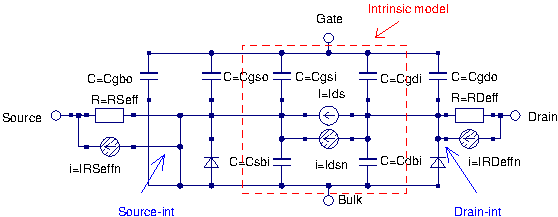
\includegraphics[width=0.9\linewidth]{EKV_Fig1}
  \caption{Equivalent circuit for the Qucs EKV v2.6 long channel nMOS model}
  \label{fig:EKV1}
\end{figure} 

\tutsubsection{Long channel model parameters (LEVEL = 1)}
\begin{scriptsize}
\begin{longtable}{ccllcc}

Name & Symbol & Description & Unit & Default nMOS & Default pMOS \\

\hline
\endhead
LEVEL &   &  Model selector    &        &  $1$       &  $1$       \\
L   & $L$ & length parameter   & $m$    & $10e-6$ & $10e-6$ \\
W   & $W$ & width parameter    & $m$    & $10e-6$ & $10e-6$ \\
Np  & $Np$ & parallel multiple device number  &   & $1$ & $1$ \\
Ns  & $Ns$ & series multiple device number    &   & $1$ & $1$ \\
Cox & $Cox$ & gate oxide capacitance per unit area   & $F/m^2$    & $3.4e-3$ & $3.4e-3$ \\
Xj  & $Xj$ & metallurgical junction length   & $m$    & $0.15e-6$ & $0.15e-6$ \\
Dw  & $Dw$ & channel width correction   & $m$    & $-0.02e-6$ & $-0.02e-6$ \\
Dl  & $Dl$ & channel length correction  & $m$    & $-0.05e-6$ & $-0.05e-6$ \\
Vto & $Vto$ & long channel threshold voltage   & $V$    & $0.5$ & $-0.55$ \\
Gamma  & $Gamma$ & body effect parameter   & $\sqrt{V}$    & $0.7$ & $0.69$ \\
Phi  & $Phi$ & bulk Fermi potential  & $V$    & $0.5$ & $0.87$ \\
Kp   & $Kp$ & transconductance parameter   & $A/V^2$    & $50e-6$ & $20e-6$ \\
Theta & $Theta$ & mobility reduction coefficient  & $1/V$    & $50e-3$ & $50e-3$ \\
Tcv  & $Tcv$ & threshold voltage temperature coefficient  & $V/K$     & $1.5e-3$ & $-1.4e-3$ \\
Hdif   & $Hdif$ & heavily doped diffusion length   & $m$    & $0.9e-6$ & $0.9e-6$ \\
Rsh & $Rsh$ & drain-source diffusion sheet resistance  &  $\Omega/square$  & $510$ & $510$ \\
Rsc  & $Rsc$ & source contact resistance  & $\Omega$     & $0.0$ & $0.0$ \\
Rdc  & $Rdc$ & drain contact resistance   & $\Omega$    & $0.0$ & $0.0$ \\
Cgso  & $Cgso$ & gate to source overlay capacitance  &  $F$  & $1.5e-10$ & $1.5e-10$ \\
Cgdo  & $Cgdo$ & gate to drain overlay capacitance  &  $F$  & $1.5e-10$ & $1.5e-10$ \\
Cgbo  & $Cgbo$ & gate to bulk overlay capacitance  &  $F$  & $4e-10$ & $4e-10$ \\
N  & $N$ & diode emission coefficient  &    & $1.0$ & $1.0$ \\
Is  & $Is$ & leakage current  & $A$   & $1e-1$ & $1e-14$ \\
Bv  & $Bv$ & reverse breakdown voltage  &  $V$  & $100$ & $100$ \\
Ibv & $Ibv$ & current at Bv  &  $A$   & $1e-3$ & $1e-3$ \\
Vj  & $Vj$ & junction potential  & $V$   & $1.0$ & $1.0$ \\
Cj0  & $Cj0$ & zero bias depletion capacitance  &  $F$  & $1e-12$ & $1e-12$ \\
M    & $M$ & grading coefficient  &     & $0.5$ & $0.5$ \\
Area & $Area$ & relative area  &    & $1.0$ & $1.0$ \\
Fc & $Fc$ & forward-bias depletion capcitance coefficient  &  & $0.5$ & $0.5$ \\
Tt  & $Tt$ & transit time  & $s$   & $0.1e-9$ & $0.1e-9$ \\
Xti  & $Xti$ & saturation current temperature exponent  &    & $3.0$ & $3.0$ \\
Kf   & $KF$  & flicker noise coefficient                &    & $1e-27$ & $1e-28$ \\
Af   & $Af$  & flicker noise exponent                   &    & $1.0$ & $1.0$ \\
Tnom & $Tnom$ & parameter measurement temperature  & $\degree C$    & $26.85$ & $26.85$ \\
Temp & $Temp$ & device temperature  & $\degree C$   & $26.85$ & $26.85$ \\

\end{longtable}
\end{scriptsize}

\tutsubsection{Fundamental long channel DC model equations (LEVEL = 1)}
<22>  \hspace{10mm} $Vg = V(Gate)-V(Bulk)$

<23>  \hspace{10mm} $Vs=V(Source)-V(Bulk)$

<24> \hspace{10mm}  $Vd=V(Drain)-V(Bulk)$

<33> \hspace{10mm}  $VGprime = Vg-Vto+Phi+Gamma \cdot \sqrt{Phi}$

<34> \hspace{10mm}  $Vp=VGprime-Phi-Gamma \cdot \left(\sqrt{VGprime+\left[ \dfrac{Gamma}{2}\right]^{2} } -\dfrac{Gamma}{2} \right) $

<39> \hspace{10mm}  $n=1 + \dfrac{Gamma}{2 \cdot \sqrt{Vp+Phi+4 \cdot Vt}}$

<58, 64> \hspace{7mm} $\beta =Kp \cdot \dfrac{W}{L} \cdot \dfrac{1}{1+Theta \cdot Vp}$

<44>  \hspace{10mm}  $X1=\dfrac{Vp-Vs}{Vt}$  \hspace{5mm}  $If = \left[ ln\left\lbrace 1+limexp\left( \dfrac{X1}{2}\right) \right\rbrace \right]^{2} $

<57>  \hspace{10mm}  $X2=\dfrac{Vp-Vd}{Vt}$  \hspace{5mm}  $Ir = \left[ ln\left\lbrace 1+limexp\left( \dfrac{X2}{2}\right) \right\rbrace \right]^{2} $

<65> \hspace{10mm}   $Ispecific = 2 \cdot n \cdot \beta \cdot Vt^{2}$

<66> \hspace{10mm}   $ Ids = Ispecific \cdot \left( If-Ir \right ) $

\vspace{8mm}

Where \textit{VGprime} is the effective gate voltage, \textit{Vp} is
the pinch-off voltage, \textit{n} is the slope factor, $\beta$ is a
transconductance parameter, \textit{Ispecific} is the specific
current, \textit{If} is the forward current, \textit{Ir} is the
reverse current, \textit{Vt} is the thermal voltage at the device
temperature, and \textit{Ids} is the drain to source current.  EKV
v2.6 equation numbers are given in ``< >'' brackets at the left-hand
side of each equation.  Typical plots of Ids against Vds for both the
nMOS and pMOS long channel devices are given in Figure~\ref{fig:EKV2}.


\begin{figure}
  \centering
  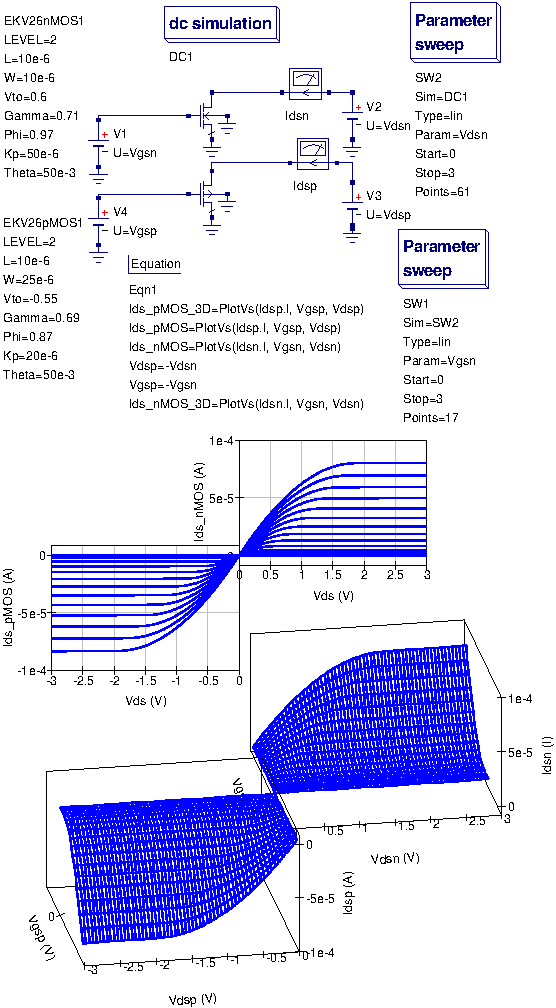
\includegraphics[width=0.7\linewidth]{EKV_Fig2}
  \caption{Ids versus Vds plots for the Qucs EKV v2.6 long channel nMOS and pMOS models}
  \label{fig:EKV2}
\end{figure} 


\tutsection{Testing model performance}

Implementing advanced component models like the EKV v2.6 MOSFET model
is a complex process, involving the translation of a set of equations
into the Verilog-A hardware design language, conversion of the
Verilog-A code into C++ code via the ADMS compiler, and finally
compiling and linking the model code with the main body of Qucs
code. At all stages in the process accuracy becomes an important
issue. This section of the Qucs EKV v2.6 report introduces a number of
test simulations which were used during the model development cycle to
check the performance of the Qucs EKV v2.6 implementation.  The tests
also demonstrate how a circuit simulator can be used to extract model
parameters. The values of which help to confirm correct model
operation.

\tutsubsection{Extraction of Ispec}

When a MOS transistor is operating in the saturation region, reverse
current \textit{Ir} approaches zero and the drain to source current is
approximated by

\hspace{20mm}     \begin{equation}
              Ids = Ispecific \cdot If = Ispecific \cdot \left[ ln\lbrace  1+limexp\left( \dfrac{Vp-Vs}{2 \cdot Vt} \right) \rbrace  \right]^{2} 
                  \end{equation}  



In saturation $limexp\left( \frac{Vp-Vs}{2 \cdot Vt} \right) >> 1$,
yielding

\hspace{20mm}     \begin{equation}
			\sqrt{Ids} = \sqrt{\dfrac{Ispecific}{2 \cdot Vt^{2}}} \cdot \left( Vp-Vs\right) 
                  \end{equation}  

Hence   
\hspace{20mm}     \begin{equation}
			\dfrac{\partial(\sqrt{Ids})}{\partial Vs} = -\sqrt{\dfrac{Ispecific}{2 \cdot Vt^{2}}} = -slope
                  \end{equation}  
Or 
\hspace{20mm}     \begin{equation}
			Ispecific = 2 \cdot slope^{2} \cdot Vt^{2}
                  \end{equation}  

Figure~\ref{fig:EKV3} shows a typical test circuit configuration for
measuring and simulating \textit{Ids} with varying \textit{Vs}. Qucs
post-simulation functions in equation block Eqn1 are used to calculate
the value for \textit{Ispecific}. The value of \textit{Ispecific} for
the nMOS transistor with the parameters given in Fig.~\ref{fig:EKV3}
is 3.95e-8 A. Figure~\ref{fig:EKV4} illustrates a test circuit for
measuring \textit{Vp} with the transistor in saturation. In this
circuit \textit{Is=Ispecific} and the threshold voltage corresponds to
\textit{Vg} when\textit{ Vp} = 0V.  Notice also that $n=\partial Vg/\partial
Vp$. In Fig.~\ref{fig:EKV4} Qucs post-simulation processing functions 
are also used to generate data for \textit{Vp},
\textit{VGprime} and \textit{n}. The value of the threshold voltage
for the device shown in Fig.~\ref{fig:EKV4} is 0.6V. At this voltage n
= 1.37. The two test configurations illustrated in
Figs.~\ref{fig:EKV3} and \ref{fig:EKV4} go some way to confirming that
the Qucs implementation of the EKV v2.6 long channel model is
functioning correctly.


\begin{figure} 
  \centering
  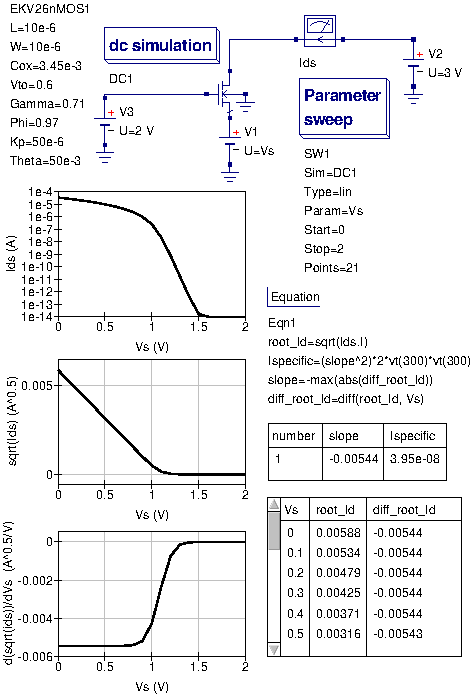
\includegraphics[width=0.8\linewidth]{EKV_Fig3}
  \caption{Ispecific extraction test circuit and post simulation data processing results}
  \label{fig:EKV3}
\end{figure} 
\begin{figure}
  \centering
  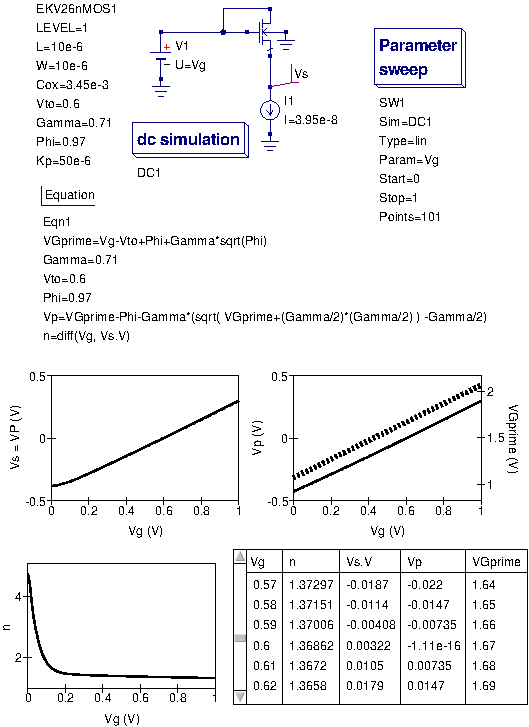
\includegraphics[width=0.8\linewidth]{EKV_Fig4}
  \caption{Vp extraction test circuit and post simulation data processing results}
  \label{fig:EKV4}
\end{figure} 


\tutsubsection{Extraction of model intrinsic capacitance}
The Qucs implementation of the EKV v2.6 MOSFET model uses the
charge-based model for transcapacitances. This model ensures
charge-conservation during transient analysis. Both the long channel
and short channel versions employ the quasi-static charge-based
model. The EKV v2.6 charge equations for the long channel intrinsic
device are:

\hspace{20mm}     \begin{equation}
			nq = 1+\dfrac{Gamma}{2 \cdot \sqrt{Vp+Phi+1e-6}}
                  \end{equation}  

\hspace{20mm}     \begin{equation}
			Xf = \sqrt{\dfrac{1}{4} + If}
                  \end{equation}  

\hspace{20mm}     \begin{equation}
			Xr = \sqrt{\dfrac{1}{4} + Ir}
                  \end{equation}  

\hspace{20mm}     \begin{equation}
			qD=-nq \cdot \left\lbrace  \dfrac{4}{15} \cdot \dfrac{3 \cdot Xr^{3} + 6 \cdot Xr^{2} \cdot Xf + 4 \cdot Xr \cdot Xf^{2} +2 \cdot Xf^{3} } { (Xf+Xr)^{2} } -\dfrac{1}{2} \right\rbrace  
                  \end{equation}  

\hspace{20mm}     \begin{equation}
			qS=-nq \cdot \left\lbrace  \dfrac{4}{15} \cdot \dfrac{3 \cdot Xf^{3} + 6 \cdot Xf^{2} \cdot Xr + 4 \cdot Xf \cdot Xr^{2} +2 \cdot Xr^{3} } { (Xf+Xr)^{2} } -\dfrac{1}{2} \right\rbrace  
                  \end{equation}  

\hspace{20mm}     \begin{equation}
			qI = qS+qD = -nq \cdot \left\lbrace  \dfrac{4}{3} \cdot \dfrac{3 \cdot Xf^{3} +  Xr \cdot Xf + Xr^{2} } { Xf+Xr } - 1 \right\rbrace  
                  \end{equation}  

\hspace{20mm}     \begin{equation} 
			qB = -Gamma \cdot \sqrt{Vp+Phi+1e-6} \cdot \dfrac{1}{
Vt} - \left( \dfrac{nq-1}{nq} \right) \cdot qI \hspace{5mm} \forall (VGprime > 0 )			
                  \end{equation}  

\hspace{20mm}     \begin{equation}
			qB = -VGprime \cdot \dfrac{1}{Vt} \hspace{5mm}\forall (VGprime <= 0 )
                  \end{equation}  

\hspace{20mm}     \begin{equation}
			qG = -qI - qB
                  \end{equation}  

\hspace{20mm}     \begin{equation}
			COX = Cox \cdot Np \cdot Weff \cdot Ns \cdot Leff
                  \end{equation}  

\hspace{20mm}     \begin{equation}
			Q(I,B,D,S,G) = COX \cdot Vt \cdot q(I,B,D,S,G)
                  \end{equation}  

The first release of the Qucs EKV v2.6 MOSFET model assumes that the
gate and bulk charge is partitioned between the drain and source in
equal ratio\footnote{For an example of this type of charge
partitioning see F. Pregaldiny et. al., An analytic quantum model for
the surface potential of deep-submicron MOSFETS, 10th International
Conference, MIXDES 2003, Lodz, Poland, 26-28 June 2003.}. Fifty
percent charge portioning yields the following \textit{Ids} current
contributions:
\hspace{20mm}     \begin{equation} 
			I(Gate, Source\_int) <+ 0.5 \cdot p\_n\_MOS \cdot ddt(QG)
                  \end{equation}  

\hspace{20mm}     \begin{equation}
			I(Gate, Drain\_int) <+ 0.5 \cdot p\_n\_MOS \cdot ddt(QG)
                  \end{equation}  

\hspace{20mm}     \begin{equation}
			I(Source\_int, Bulk) <+ 0.5 \cdot p\_n\_MOS \cdot ddt(QB)
                  \end{equation} 

\hspace{20mm}     \begin{equation}
			I(drain\_int, Bulk) <+ 0.5 \cdot p\_n\_MOS \cdot ddt(QB)
                  \end{equation}  


\vspace{8mm}
Where p\_n\_MOS = 1 for nMOS devices or -1 for pMOS devices. Charge
associated with the extrinsic overlap capacitors, Cgs0, Cgd0 and Cgb0,
is represented in the Qucs EKV v2.6 implementation by the following
equations:

\hspace{20mm}     \begin{equation} 
			Qgs0 = Cgs0 \cdot Weff \cdot Np \cdot (VG - VS)
                  \end{equation}  

\hspace{20mm}     \begin{equation} 
			Qgd0 = Cgd0 \cdot Weff \cdot Np \cdot (VG - VD)
                  \end{equation}  

\hspace{20mm}     \begin{equation} 
			Qgb0 = Cgb0 \cdot Leff \cdot Np \cdot VB
                  \end{equation}  

The drain to bulk and source to bulk diodes also introduce additional
components in the extrinsic capacitance model. The default value of
CJ0 being set at 300fF.  Analysis of the y-parameters\footnote{A more
detailed anlysis of the EKV v2.6 y-parameters can be found in
F. Krummenacher \textit{et. al.}, HF MOSET MODEL parameter extraction,
European Project No. 25710, Deliverable D2.3, July 28, 2000.} for the
EKV v2.6 equivalent circuit shown in the test circuit illustrated in
Fig.~\ref{fig:EKV5} yields

\hspace{20mm}     \begin{equation} 
			y_{11} = \dfrac{j \cdot \omega \cdot Cg}{1+\omega^{2} \cdot (Rgn \cdot Cg)^{2}}
                  \end{equation}  
Or
\hspace{20mm}     \begin{equation} 
			y_{11} \cong \omega^{2} \cdot Rg \cdot Cg^{2} + j \cdot \omega \cdot Cg, \hspace{3mm} \textrm{when} \hspace{3mm} \omega \cdot Rg \cdot Cg << 1.
                  \end{equation}  

Hence, $ Cg = imag( y_{11}/ \omega)$ and $Rgn = real( y_{11}/(
\omega^{2} \cdot Cg^{2}))$, where $\omega = 2 \cdot \pi \cdot f$, and $f$
is the frequency of y-parameter measurement, Rg is a series extrinsic
gate resistance and $Cg \cong Cgs + Cgd + Cgb$.  With equal
partitioning of the intrinsic gate charge $Cgb$ approximates to zero
and $Cg \cong Cgs + Cgd$. The data illustrated in
Figures~\ref{fig:EKV5} and ~\ref{fig:EKV6} shows two features which
are worth commenting on; firstly the values of Cg are very much in
line with simple hand calculations (for example in the case of the
nMOS device $Cg(max) = W \cdot L \cdot Cox = 10e-6 * 10e-6* 3.45e-3 =
3.45e-13$F) and secondly both sets of simulation data indicate the
correct values for the nMOS and pMOS threshold voltages (for example
-0.55 V for the pMOS device and 0.6 V for the nMOS device),
reinforcing confidence in the EKV v2.6 model implementation.

\begin{figure} 
  \centering
  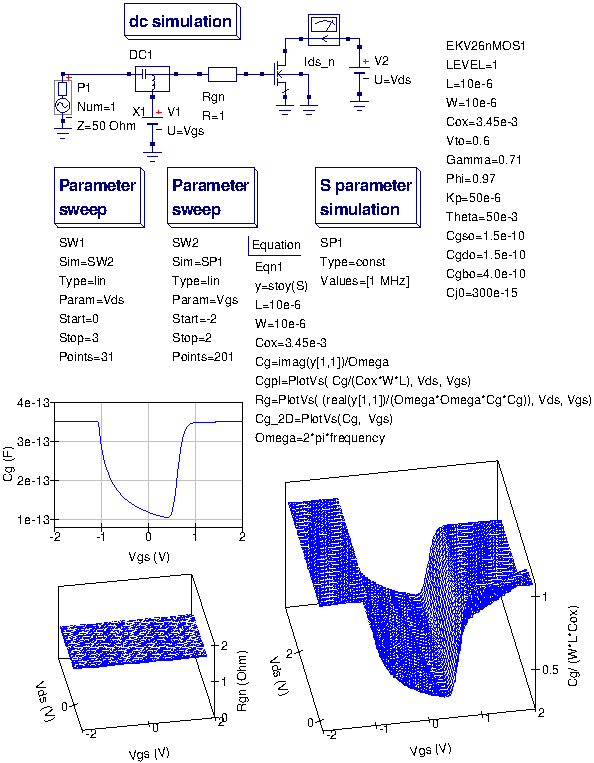
\includegraphics[width=0.8\linewidth]{EKV_Fig5}
  \caption{$\mathrm{y_{11}}$ test circuit and values of Cg for the long channel EKV v2.6 nMOS model}
  \label{fig:EKV5}
\end{figure} 
\begin{figure}
  \centering
  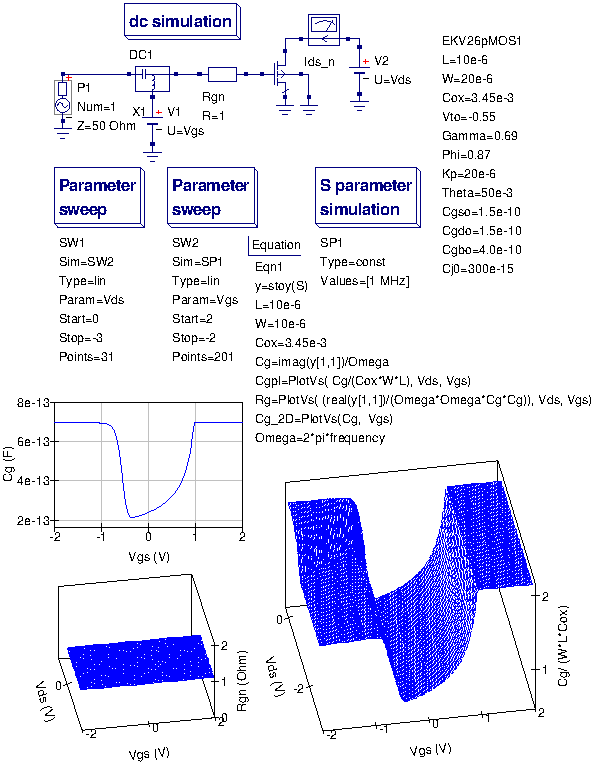
\includegraphics[width=0.8\linewidth]{EKV_Fig6}
  \caption{$\mathrm{y_{11}}$ test circuit and values of Cg for the long channel EKV v2.6 pMOS model}
  \label{fig:EKV6}
\end{figure}  



\tutsubsection{Extraction of extrinsic diode capacitance and drain resistance}

The extrinsic section of the EKV v2.6 model includes diodes which in
turn are modelled by conventional DC characteristics and parallel
capacitance.  This capacitance is represented by depletion layer
capacitance in the diode reverse bias region of operation.  In the
diode forward bias section of the I-V characteristic diffusion
capacitance dominates. Figure~\ref{fig:EKV7} illustrates a test
circuit that allows the diode capacitance to be extracted as a
function of \textit{Vds}. In Fig.~\ref{fig:EKV7} the nMOS device is
turned off and the drain to bulk diode reverse biased. Simple analysis
indicates that

\hspace{20mm}     \begin{equation} 
			y_{11} \cong \omega^{2} \cdot RDeff \cdot Cd^{2} + j \cdot \omega \cdot Cd, \hspace{3mm} \textrm{when} \hspace{3mm} \omega \cdot RDeff \cdot Cd << 1.
                  \end{equation}  

Hence, $ Cd = imag( y_{11}/ \omega)$ and $Rdeff = real( y_{11}/(
\omega^{2} \cdot Cd^{2}))$, where $\omega = 2 \cdot \pi \cdot f$, $f$ is
the frequency of y-parameter measurement, and $Cd$ is the diode
capacitance. The data shown in Fig.~\ref{fig:EKV7} indicate good
agreement with the expected values for \textit{Cd} and \textit{RDeff};
which are expected to be \textit{Cd} = 300fF at \textit{Vds}=0V, and
\textit{Rdeff} = 46$\Omega$.
 
\begin{figure}
  \centering
  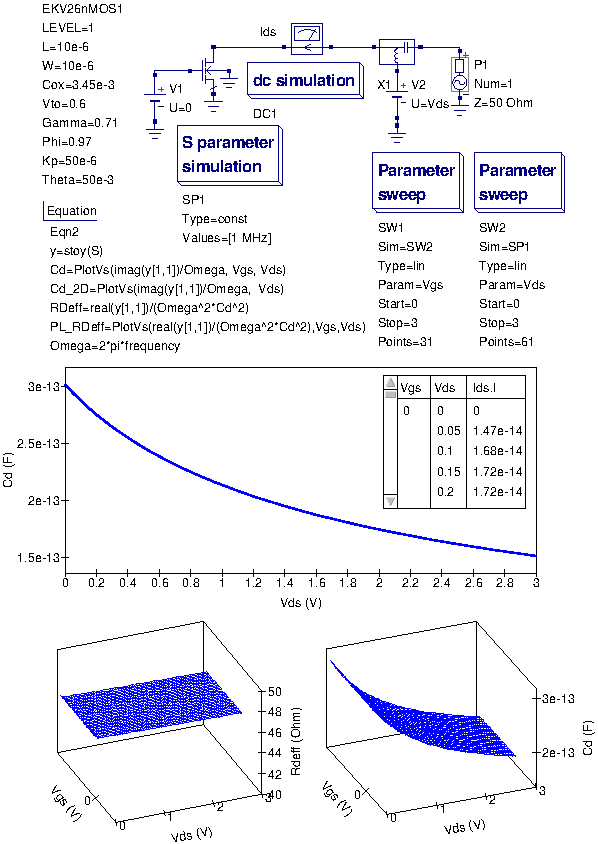
\includegraphics[width=0.8\linewidth]{EKV_Fig7}
  \caption{Test circuit for extracting EKV v2.6 extrinsic diode capacitance}
  \label{fig:EKV7}
\end{figure}  


\tutsubsection{Simulating EKV v2.6 MOSFET noise}

The EKV v2.6 intrinsic device noise is modelled by a noise current
source connected between the internal drain and source terminals. The
noise current source \textit{Idsn}, see Fig.~\ref{fig:EKV1}, is
composed of a thermal noise component and a flicker noise
component. The Power Spectral Density ($S_{PSD}$) of these components
are given by:

\hspace{20mm}     \begin{equation} 
			S_{PSD} = S_{thermal} + S_{flicker}
                  \end{equation}  

Where
\begin{itemize}
 \item  Thermal noise
\hspace{20mm}     \begin{equation} 
			S_{thermal}=4 \cdot k \cdot T \cdot \beta \cdot \mid qI \mid
                  \end{equation}  
 \item Flicker noise
\hspace{20mm}     \begin{equation} 
		     S_{flicker} = \dfrac{KF \cdot g_{mg}^{2}}{Np \cdot Weff \cdot Ns \cdot Leff \cdot Cox \cdot f^{Af}},
                  \end{equation}
\hspace{20mm}     \begin{equation} 
		     g_{mg} = \dfrac{\partial Ids}{\partial Vgs} = \beta \cdot Vt \cdot \left( \sqrt{\dfrac{4 \cdot If}{Ispecific}+1}-\sqrt{\dfrac{4 \cdot Ir}{Ispecific}+1} \right) 
                  \end{equation}  
		
\end{itemize}

Where $\beta $ is a transconductance factor, $qI=qD+qS$, and the other
symbols are defined in the EKV v2.6 long channel parameter list or
have their usual meaning. Noise has been implemented in both the Qucs
long channel and short channel EKV v2.6 models. In addition to the
intrinsic device noise the Qucs EKV v2.6 model includes the thermal
noise components for both extrinsic resistors \textit{RDeff} and
\textit{RSeff}. Figure~\ref{fig:EKV8} presents a typical noise test
circuit and simulated noise currents. In Figure~\ref{fig:EKV8} four
nMOS devices are biased under different DC conditions and their noise
current simulated for a range of \textit{W} values between 1e-6 m and
100e-6 m. The first three devices include both thermal and flicker
noise components (\textit{KF} = 1e-27) while the fourth device has
it's flicker component set to zero. The resulting current noise curves
clearly demonstrate the effect of summing intrinsic thermal and
flicker components on the overall performance of the EKV v2.6 noise
model.

\begin{figure}
  \centering
  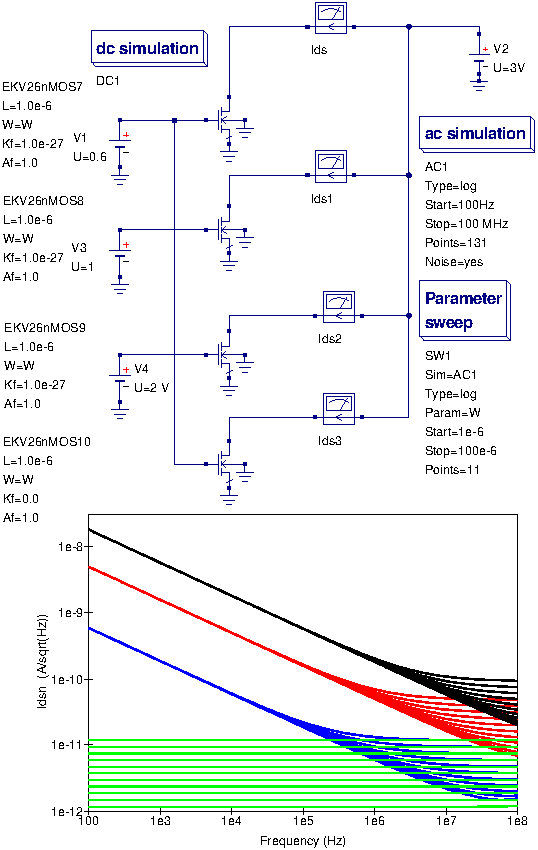
\includegraphics[width=0.5\linewidth]{EKV_Fig8}
  \caption{Test circuit for simulating EKV v2.6 noise: Ids.in blue curve, Ids1.in red curve, Ids2.in black curve and Ids3.in green curve }
  \label{fig:EKV8}
\end{figure}  


\tutsection{The Qucs short channel EKV v2.6 model}

The Qucs implementation of the short short channel EKV v2.6 MOSFET
model contains all the features implemented in the long channel
version of the model plus a number of characteristics specific to
short channel operation. However, the short channel version of the
model does not use parameter \textit{Theta}. Parameter LEVEL set to 2
selects the short channel model. Both pMOS and nMOS versions of the
model are available for both long and short channel implementations.
The entire short channel EKV v2.6 MOSFET model is described by roughly
94 equations. Readers who are interested in the mathematics of the
model should consult ``The EPFL-EKV MOSFET Model Equations for
Simulation'' publication cited in previous text.  Appendix A lists the
complete Verilog-A code for the first release of the Qucs EKV v2.6
MOSFET models.  Additional Verilog-A code has been added to the model
equation code to (1) allow interchange of the drain and source
terminals, and (2) select nMOS or pMOS devices.

\tutsubsection{Short channel model parameters (LEVEL = 2)}
\begin{scriptsize}
\begin{longtable}{ccllcc}

Name & Symbol & Description & Unit & Default nMOS & Default pMOS \\

\hline
\endhead
LEVEL &   &  Model selector    &        &  $2$       &  $2$       \\
L   & $L$ & length parameter   & $m$    & $10e-6$ & $10e-6$ \\
W   & $W$ & width parameter    & $m$    & $10e-6$ & $10e-6$ \\
Np  & $Np$ & parallel multiple device number  &   & $1$ & $1$ \\
Ns  & $Ns$ & series multiple device number    &   & $1$ & $1$ \\
Cox & $Cox$ & gate oxide capacitance per unit area   & $F/m^2$    & $3.4e-3$ & $3.4e-3$ \\
Xj  & $Xj$ & metallurgical junction length   & $m$    & $0.15e-6$ & $0.15e-6$ \\
Dw  & $Dw$ & channel width correction   & $m$    & $-0.02e-6$ & $-0.02e-6$ \\
Dl  & $Dl$ & channel length correction  & $m$    & $-0.05e-6$ & $-0.05e-6$ \\
Vto & $Vto$ & long channel threshold voltage   & $V$    & $0.5$ & $-0.55$ \\
Gamma  & $Gamma$ & body effect parameter   & $\sqrt{V}$    & $0.7$ & $0.69$ \\
Phi  & $Phi$ & bulk Fermi potential  & $V$    & $0.5$ & $0.87$ \\
Kp   & $Kp$ & transconductance parameter   & $A/V^2$    & $50e-6$ & $20e-6$ \\
EO & $EO$ & mobility reduction coefficient   & $V/m$    & $88e-6$ & $51e-6$ \\
Ucrit  & $Ucrit$ & longitudinal critical field   & $V/m$    & $4.5e-6$ & $18e-6$ \\
Lambda  & $Lambda$ & depletion length coefficient  &     & $0.23$ & $1.1$ \\
Weta & $Weta$ & narrow channel effect coefficient   &     & $0.05$ & $0.0$ \\
Leta  & $eta$ & short channel effect coefficient   &     & $0.28$ & $0.45$ \\
Q0 & $Q0$ & reverse short channel effect peak charge density  &     & $280e-6$ & $200e-6$ \\
Lk   & $Lk$ & reverse short channel effect characteristic length   & $m$    & $0.5e-6$ & $0.6e-6$ \\
Tcv  & $Tcv$ & threshold voltage temperature coefficient  & $V/K$     & $1.5e-3$ & $-1.4e-3$ \\
Bex & $Bex$ & mobility temperature coefficient  &     & $-1.5$ & $-1.4$ \\
Ucex   & $Ucex$ & longitudinal critical field temperature exponent   & $ $    & $1.7$ & $2.0$ \\
Ibbt  & $Ibbt$ & temperature coefficient for Ibb  & $1/K$     & $0.0$ & $0.0$ \\
Hdif   & $Hdif$ & heavily doped diffusion length   & $m$    & $0.9e-6$ & $0.9e-6$ \\
Rsh & $Rsh$ & drain-source diffusion sheet resistance  &  $\Omega/square$  & $510$ & $510$ \\
Rsc  & $Rsc$ & source contact resistance  & $\Omega$     & $0.0$ & $0.0$ \\
Rdc  & $Rdc$ & drain contact resistance   & $\Omega$    & $0.0$ & $0.0$ \\
Cgso  & $Cgso$ & gate to source overlay capacitance  &  $F$  & $1.5e-10$ & $1.5e-10$ \\
Cgdo  & $Cgdo$ & gate to drain overlay capacitance  &  $F$  & $1.5e-10$ & $1.5e-10$ \\
Cgbo  & $Cgbo$ & gate to bulk overlay capacitance  &  $F$  & $4e-10$ & $4e-10$ \\
N  & $N$ & diode emission coefficient  &    & $1.0$ & $1.0$ \\
Is  & $Is$ & leakage current  & $A$   & $1e-1$ & $1e-14$ \\
Bv  & $Bv$ & reverse breakdown voltage  &  $V$  & $100$ & $100$ \\
Ibv & $Ibv$ & current at Bv  &  $A$   & $1e-3$ & $1e-3$ \\
Vj  & $Vj$ & junction potential  & $V$   & $1.0$ & $1.0$ \\
Cj0  & $Cj0$ & zero bias depletion capacitance  &  $F$  & $1e-12$ & $1e-12$ \\
M    & $M$ & grading coefficient  &     & $0.5$ & $0.5$ \\
Area & $Area$ & relative area  &    & $1.0$ & $1.0$ \\
Fc & $Fc$ & forward-bias depletion capcitance coefficient  &  & $0.5$ & $0.5$ \\
Tt  & $Tt$ & transit time  & $s$   & $0.1e-9$ & $0.1e-9$ \\
Xti  & $Xti$ & saturation current temperature exponent  &    & $3.0$ & $3.0$ \\
Kf   & $KF$  & flicker noise coefficient                &    & $1e-27$ & $1e-28$ \\
Af   & $Af$  & flicker noise exponent                   &    & $1.0$ & $1.0$ \\
Avto  & $Avto$ & area related threshold mismatch parameter  &    & $0$ & $0$ \\
Akp   & $Akp$  & area related gain mismatch parameter       &    & $0$ & $0$ \\
Agamma   & $Agamma$  & area related body effect mismatch parameter &    & $0$ & $0$ \\
Iba  & $Iba$ & first impact ionization coefficient  & $1/m$   & $2e8$ & $0.0$ \\
Ibb   & $Ibb$  & second impact ionization coefficient & $V/m$    & $3.5e8$ & $3.5e8$ \\
Ibn   & $Ibn$  & saturation voltage factor for impact ionization  &    & $1.0$ & $1.0$ \\
Tnom & $Tnom$ & parameter measurement temperature  & $\degree C$    & $26.85$ & $26.85$ \\
Temp & $Temp$ & device temperature  & $\degree C$   & $26.85$ & $26.85$ \\

\end{longtable}
\end{scriptsize}

\tutsubsection{Simulating short channel charge sharing effects}

A simple test circuit for demonstrating the effects of charge sharing
is given in Figure~\ref{fig:EKV9}. With charge sharing disabled, by
setting Weta and Leta to zero, the magnitude and slope of the
\textit{Ids} vs. \textit{Vds} curve shows a marked difference to that
where charge sharing is enabled.  One point to note with this test:
charge sharing in short channel devices significantly reduces the
device output resistance which could have, of course, important
consequences on circuit performance.

\begin{figure}
  \centering
  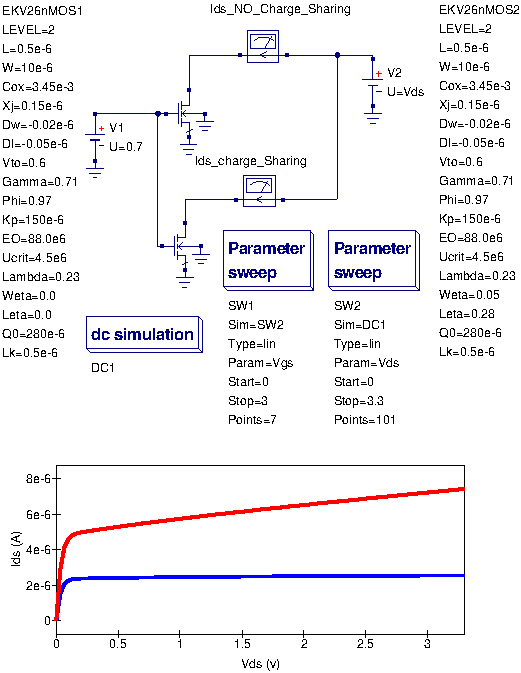
\includegraphics[width=0.5\linewidth]{EKV_Fig9}
  \caption{Test circuit for simulating EKV v2.6 charge sharing effects in short channel devices: \textit{Ids} blue curve; NO charge sharing (\textit{Weta} = 0.0, \textit{Leta} = 0.0), \textit{Ids} red curve; charge sharing (\textit{Weta} = 0.05, \textit{Leta} = 0.28)}
  \label{fig:EKV9}
\end{figure}  

\tutsection{End note}

This report outlines some of the background to the Qucs implementation
of the EKV v2.6 MOSFET model. A series of test results demonstrate a
range of results that have been achieved with this new Qucs compact
device model. Although the test results give data similar to what is
expected in all cases it must be stressed that this is the first
release of this MOSFET model and as such it will probably contain
bugs. A great deal of work has gone into providing this new Qucs
model. However, all the effort has been worthwhile because for the
first time Qucs now has a submicron MOSFET model. Please use the model
and report bugs to the Qucs development team. Much work still remains
to be done in the development of MOSFET models for Qucs. In future
releases both bug fixes and new models are likely to feature
strongly. Once again I would like to thank Stefan Jahn and W\l adys\l
aw Grabi\'{n}ski (of MOS-AK) for their encouragement and support
during the period I have been working on developing the Qucs
implementation of the EKV v2.6 model and writing this report.

\tutsection{Qucs Verilog-A code for the EKV v2.6 MOSFET model}

\tutsubsection{nMOS: EKV equation numbers are given on the right-hand side of code lines}
\begin{lstlisting}[
  language=Verilog,
  basicstyle=\scriptsize]
//   Qucs EPFL-EKV 2.6 nMOS model:
//
//   The structure and theoretical background to the EKV 2.6
//   Verilog-a model is presented in the Qucs EPFL-EKV 2.6 report.
//   Typical parameters are for 0.5um CMOS (C) EPLFL-LEG 1999.
//   Geometry range: Short channel W >= 0.8um, L >= 0.5um
//                   Long channel  W >= 2um,   L >= 2um
//   Voltage range:  |Vgb| < 3.3V, |Vdb| < 3.3V, |Vsb| < 2V
//
//   This is free software; you can redistribute it and/or modify
//   it under the terms of the GNU General Public License as published by
//   the Free Software Foundation; either version 2, or (at your option)
//   any later version.
// 
//   Copyright (C), Mike Brinson, mbrin72043@yahoo.co.uk, May 2008.
//
`include "disciplines.vams"
`include "constants.vams"

// 
 module EKV26nMOS (Drain, Gate, Source, Bulk);
 inout Drain, Gate, Source, Bulk;
electrical Drain, Gate, Source, Bulk;
// Internal nodes
electrical Drain_int, Source_int;
`define attr(txt) (*txt*)
// Device dimension parameters
 parameter real LEVEL = 1 from [1 : 2]  
	`attr(info="long = 1, short = 2");
 parameter real L = 0.5e-6 from [0.0 : inf]  
	`attr(info="length parameter" unit = "m" );
 parameter real W = 10e-6 from [0.0 : inf]  
	`attr(info="Width parameter" unit = "m"); 
 parameter real Np = 1.0 from [1.0 : inf]   
	`attr(info="parallel multiple device number");
 parameter real Ns = 1.0 from [1.0 : inf] 
	`attr(info="series multiple device number"); 
// Process parameters
 parameter real Cox = 3.45e-3 from [0 : inf]         
	`attr(info="gate oxide capacitance per unit area" unit = "F/m**2" );
 parameter real Xj = 0.15e-6 from [0.01e-6 : 1.0e-6] 
	`attr(info="metallurgical junction depth" unit = "m");
 parameter real Dw = -0.02e-6 from [-inf : 0.0]      
	`attr(info="channel width correction" unit = "m");
 parameter real Dl = -0.05e-6 from [-inf : 0.0]       
	`attr(info="channel length correction" unit = "m");
// Basic intrinsic model parameters
 parameter real Vto = 0.6 from [1e-6 : 2.0]         
	`attr(info="long channel threshold voltage" unit="V" );
 parameter real Gamma = 0.71 from [0.0 : 2.0]       
	`attr(info="body effect parameter" unit="V**(1/2)");
 parameter real Phi = 0.97 from [0.3 : 2.0]         
	`attr(info="bulk Fermi potential" unit="V");
 parameter real Kp = 150e-6 from [10e-6 : inf]      
	`attr(info="transconductance parameter" unit = "A/V**2");
 parameter real Theta = 50e-3 from [0.0 : inf]      
	`attr(info="mobility reduction coefficient" unit = "1/V");
 parameter real EO = 88.0e6 from [1.0e6 : inf]      
	`attr(info="mobility coefficient" unit="V/m");
 parameter real Ucrit = 4.5e6 from [2.0e6 : 25.0e6] 
	`attr(info="longitudinal critical field" unit="V/m");
// Channel length and charge sharing parameters
 parameter real Lambda = 0.23 from [0.1 : inf]      
	`attr(info="depletion length coefficient");
 parameter real Weta = 0.05 from [0.0 : inf]        
	`attr(info="narrow-channel effect coefficient");
 parameter real Leta = 0.28 from [0.0 : inf]        
	`attr(info="longitudinal critical field");
// Reverse short channel effect parameters
 parameter real Q0 = 280e-6 from [0.0 : inf]        
	`attr(info="reverse short channel charge density" unit="A*s/m**2");
 parameter real Lk = 0.5e-6 from [0.0 : inf]        
	`attr(info="characteristic length" unit="m");
// Intrinsic model temperature parameters
 parameter real Tcv = 1.5e-3   
	`attr(info="threshold voltage temperature coefficient" unit="V/K");
 parameter real Bex = -1.5     
	`attr(info="mobility temperature coefficient");
 parameter real Ucex = 1.7     
	`attr(info="Longitudinal critical field temperature exponent");
 parameter real Ibbt = 0.0     
	`attr(info="Ibb temperature coefficient"  unit="1/K");
// Series resistance calculation parameters
 parameter real Hdif = 0.9e-6 from [0.0 :inf]  
	`attr(info="heavily doped diffusion length" unit = "m");
 parameter real Rsh = 510.0 from [0.0 : inf]   
	`attr(info="drain/source diffusion sheet resistance" unit="Ohm/square");
 parameter real Rsc = 0.0 from [0.0 : inf]     
	`attr(info="source contact resistance" unit="Ohm");
 parameter real Rdc = 0.0 from [0.0 : inf]     
	`attr(info="drain contact resistance" unit="Ohm");
// Gate overlap capacitances
 parameter real Cgso = 1.5e-10 from [0.0 :inf]  
	`attr(info="gate to source overlap capacitance" unit = "F/m");
 parameter real Cgdo = 1.5e-10 from [0.0 : inf] 
	`attr(info="gate to drain overlap capacitance"  unit=  "F/m");
 parameter real Cgbo = 4.0e-10 from [0.0 : inf] 
	`attr(info="gate to bulk overlap capacitance"   unit=  "F/m");
// Impact ionization related parameters
 parameter real Iba = 2e8 from [0.0 :inf]        
	`attr(info="first impact ionization coefficient" unit = "1/m");
 parameter real Ibb = 3.5e8 from [1.0e8 : inf]   
	`attr(info="second impact ionization coefficient" unit="V/m");
 parameter real Ibn = 1.0 from [0.1 : inf]       
	`attr(info="saturation voltage factor for impact ionization");
// Flicker noise parameters
 parameter real Kf = 1.0e-27 from [0.0 :inf]   
	`attr(info="flicker noise coefficient");
 parameter real Af = 1.0 from [0.0 : inf]      
	`attr(info="flicker noise exponent" );
// Matching parameters
 parameter real Avto = 0.0 from [0.0 :inf]     
	`attr(info="area related theshold voltage mismatch parameter" unit = "V*m");
 parameter real Akp = 0.0 from [0.0 : inf]     
	`attr(info="area related gain mismatch parameter" unit="m");
 parameter real Agamma = 0.0 from [0.0 : inf]  
	`attr(info="area related body effect mismatch parameter" unit="sqrt(V)*m");
// Diode parameters
 parameter real N=1.0 from [1e-6:inf]          
	`attr(info="emission coefficient");
 parameter real Is=1e-14 from [1e-20:inf]      
	`attr(info="saturation current" unit="A" );
 parameter real Bv=100 from [1e-6:inf]        
	`attr(info="reverse breakdown voltage" unit="V");
 parameter real Ibv=1e-3 from [1e-6:inf]       
	`attr(info="current at reverse breakdown voltage" unit="A");
 parameter real Vj=1.0 from [1e-6:inf]         
	`attr(info="junction potential" unit="V");
 parameter real Cj0=300e-15 from [0:inf]         
	`attr(info="zero-bias junction capacitance" unit="F");
 parameter real M=0.5 from [1e-6:inf]          
	`attr(info="grading coefficient");
 parameter real Area=1.0 from [1e-3:inf]       
	`attr(info="diode relative area");
 parameter real Fc=0.5 from [1e-6:inf]         
	`attr(info="forward-bias depletion capcitance coefficient");
 parameter real Tt=0.1e-9 from [1e-20:inf]     
	`attr(info="transit time" unit="s" );
 parameter real Xti=3.0 from [1e-6:inf]        
	`attr(info="saturation current temperature exponent");
// Temperature parameters
 parameter real Tnom = 26.85                   
	`attr(info="parameter measurement temperature" unit = "Celsius");
// Local variables
real epsilonsi, epsilonox, Tnomk, T2, Tratio, Vto_T, Ucrit_T, Egnom, Eg, Phi_T;
real Weff, Leff, RDeff, RSeff, con1, con2, Vtoa, Kpa,Kpa_T,Gammaa, C_epsilon, xi;
real nnn, deltaV_RSCE, Vg, Vs, Vd, Vgs, Vgd, Vds, Vdso2, VG, VS, VD;
real VGprime, VP0, VSprime, VDprime, Gamma0, Gammaprime, Vp;
real n, X1, iff, X2, ir, Vc, Vdss, Vdssprime, deltaV, Vip;
real Lc, DeltaL, Lprime, Lmin, Leq, X3, irprime, Beta0, eta;
real Qb0, Beta0prime, nq, Xf, Xr, qD, qS, qI, qB, Beta, Ispecific, Ids, Vib, Idb, Ibb_T;
real A, B, Vt_T2, Eg_T1, Eg_T2, Vj_T2, Cj0_T2, F1, F2, F3, Is_T2;
real Id1, Id2, Id3, Id4, Is1, Is2, Is3, Is4, V1, V2, Ib_d, Ib_s, Qd, Qs, Qd1, Qd2, Qs1, Qs2;
real qb, qg, qgso, qgdo, qgbo, fourkt, Sthermal, gm, Sflicker, StoDswap, p_n_MOS;
//
analog begin
// Equation initialization
p_n_MOS = 1.0; // nMOS
A=7.02e-4;
B=1108.0;
epsilonsi = 1.0359e-10;     // Eqn 4
epsilonox = 3.453143e-11;   // Eqn 5
Tnomk = Tnom+273.15;              // Eqn 6
T2=$temperature;
Tratio = T2/Tnomk;
Vto_T = Vto-Tcv*(T2-Tnomk);
Egnom = 1.16-0.000702*Tnomk*Tnomk/(Tnomk+1108);
Eg =    1.16-0.000702*T2*T2/(T2+1108);
Phi_T = Phi*Tratio - 3.0*$vt*ln(Tratio)-Egnom*Tratio+Eg;
Ibb_T = Ibb*(1.0+Ibbt*(T2 -Tnomk));
Weff = W + Dw;   // Eqn 25
Leff = L + Dl;   // Eqn 26
RDeff = ( (Hdif*Rsh)/Weff)/Np + Rdc;
RSeff = ( (Hdif*Rsh)/Weff)/Np + Rsc;
con1 = sqrt(Np*Weff*Ns*Leff);
Vt_T2=`P_K*T2/`P_Q;
Eg_T1=Eg-A*Tnomk*Tnomk/(B+Tnomk);
Eg_T2=Eg-A*T2*T2/(B+T2);
Vj_T2=(T2/Tnomk)*Vj-(2*Vt_T2)*ln(pow((T2/Tnomk),1.5))-((T2/Tnomk)*Eg_T1-Eg_T2);
Cj0_T2=Cj0*(1+M*(400e-6*(T2-Tnomk)-(Vj_T2-Vj)/Vj));
F1=(Vj/(1-M))*(1-pow((1-Fc),(1-M)));
F2=pow((1-Fc), (1+M));
F3=1-Fc*(1+M);
Is_T2=Is*pow( (T2/Tnomk), (Xti/N))*limexp((-Eg_T1/Vt_T2)*(1-T2/Tnomk));
con2 = (Cox*Ns*Np*Weff*Leff);
fourkt = 4.0*`P_K*T2;
//
if (LEVEL == 2)
 begin
  Ucrit_T = Ucrit*pow(Tratio, Ucex);
  Vtoa = Vto+Avto/con1;              // Eqn 27
  Kpa = Kp*(1.0+Akp/con1);           // Eqn 28
  Kpa_T = Kpa*pow( Tratio, Bex);     // Eqn 18
  Gammaa = Gamma+Agamma/con1;        // Eqn 29
  C_epsilon = 4.0*pow(22e-3, 2);     // Eqn 30
  xi = 0.028*(10.0*(Leff/Lk)-1.0);   // Eqn 31
  nnn = 1.0+0.5*(xi+ sqrt(pow(xi,2) + C_epsilon));
  deltaV_RSCE = (2.0*Q0/Cox)*(1.0/pow(nnn,2)); // Eqn 32
 end
//
// Model branch and node voltages
//

Vg = p_n_MOS*V(Gate, Bulk); 
Vs = p_n_MOS*V(Source, Bulk);
Vd = p_n_MOS*V(Drain, Bulk);
VG=Vg;        // Eqn 22
if ( (Vd-Vs) >= 0.0)
	begin
          StoDswap = 1.0;
	  VS=Vs;   // Eqn 23
          VD=Vd;   // Eqn 24
	end
else
	begin
          StoDswap = -1.0;
	  VD=Vs;
	  VS=Vd;
	end
if (LEVEL == 2)
    VGprime=VG-Vto_T-deltaV_RSCE+Phi_T+Gamma*sqrt(Phi_T);  // Eqn 33  nMOS equation
else
    VGprime=Vg-Vto_T+Phi_T+Gamma*sqrt(Phi_T);

//
if (LEVEL == 2)
 begin
  if (VGprime > 0)
	VP0=VGprime-Phi_T-Gammaa*(sqrt(VGprime+(Gammaa/2.0)*(Gammaa/2.0))
	     -(Gammaa/2.0));  // Eqn 34
  else
	VP0 = -Phi_T;
  VSprime=0.5*(VS+Phi_T+sqrt(pow( (VS+Phi_T),2) + pow( (4.0*$vt),2)));  // Eqn 35
  VDprime=0.5*(VD+Phi_T+sqrt(pow( (VD+Phi_T),2) + pow( (4.0*$vt),2)));  // Eqn 35
  Gamma0=Gammaa-(epsilonsi/Cox)*((Leta/Leff)*(sqrt(VSprime)+sqrt(VDprime))
               -(3.0*Weta/Weff)*sqrt(VP0+Phi_T));  // Eqn 36
  Gammaprime = 0.5*(Gamma0+sqrt( pow(Gamma0,2) +0.1*$vt ));  // Eqn 37 
  if (VGprime > 0.0 )
           Vp = VGprime-Phi_T-Gammaprime*(sqrt(VGprime+(Gammaprime/2.0)*
	        (Gammaprime/2.0)) - (Gammaprime/2.0)); // Eqn 38
  else
        Vp = -Phi_T;
  n = 1.0 +Gammaa/(2.0*sqrt(Vp+Phi_T+4.0*$vt));  // Eqn 39
 end
else
  begin
   if (VGprime > 0)
	Vp=VGprime-Phi_T-Gamma*(sqrt(VGprime+(Gamma/2.0)*(Gamma/2.0))
	   -(Gamma/2.0));  // Eqn 34
   else
	Vp = -Phi_T;
   n = 1.0 +Gamma/(2.0*sqrt(Vp+Phi_T+4.0*$vt));  // Eqn 39
end
//
X1 = (Vp-VS)/$vt;
iff = ln(1.0+limexp(X1/2.0))*ln(1.0+limexp(X1/2.0));   // Eqn 44
X2 = (Vp-VD)/$vt;
ir = ln(1.0+limexp(X2/2.0))*ln(1.0+limexp(X2/2.0));    // Eqn 57
//
if (LEVEL == 2)
 begin
   Vc = Ucrit_T*Ns*Leff;  // Eqn 45
   Vdss = Vc*(sqrt( 0.25 + (($vt/(Vc))*sqrt(iff)))-0.5);  // Eqn 46;
   Vdssprime = Vc*(sqrt( 0.25 + ($vt/Vc)*(sqrt(iff)-0.75*ln(iff))) - 0.5) 
	       +$vt*(ln(Vc/(2.0*$vt)) - 0.6 ); // Eqn 47
   if (Lambda*(sqrt(iff) > (Vdss/$vt) ) )
          deltaV = 4.0*$vt*sqrt(Lambda*(sqrt(iff) -(Vdss/$vt)) 
		   + (1.0/64.0) );  // Eqn 48
   else   
          deltaV = 1.0/64.0;
   Vdso2 = (VD-VS)/2.0;        // Eqn 49
   Vip = sqrt( pow(Vdss, 2) + pow( deltaV,2)) - sqrt( pow( (Vdso2 - Vdss), 2) 
	 + pow (deltaV, 2));  // Eqn 50
   Lc = sqrt( (epsilonsi/Cox)*Xj);  // Eqn 51
   DeltaL = Lambda*Lc*ln(1.0+((Vdso2-Vip)/(Lc*Ucrit_T)));  // Eqn 52
   Lprime = Ns*Leff - DeltaL + ( (Vdso2+Vip)/Ucrit_T); // Eqn 53
   Lmin = Ns*Leff/10.0;  // Eqn 54
   Leq = 0.5*(Lprime + sqrt( pow(Lprime, 2) + pow(Lmin, 2)));   // Eqn 55
   X3 = (Vp-Vdso2-VS-sqrt( pow(Vdssprime, 2) + pow( deltaV, 2)) 
	+ sqrt( pow( (Vdso2-Vdssprime), 2) + pow(deltaV,2)))/$vt;
   irprime = ln(1.0+limexp(X3/2.0))*ln(1.0+limexp(X3/2.0));  // Eqn 56
   Beta0 = Kpa_T*(Np*Weff/Leq);     // Eqn 58
   eta = 0.5;  // Eqn 59 - nMOS
   Qb0 = Gammaa*sqrt(Phi_T);  // Eqn 60;
   Beta0prime = Beta0*(1.0 +(Cox/(EO*epsilonsi))*Qb0);  // Eqn 61
   nq = 1.0 +Gammaa/(2.0*sqrt(Vp+Phi_T+1e-6));          // Eqn 69
 end
else
 nq = 1.0 +Gamma/(2.0*sqrt(Vp+Phi_T+1e-6));          // Eqn 69
//
Xf = sqrt(0.25+iff);    // Eqn 70
Xr = sqrt(0.25+ir);     // Eqn 71
qD = -nq*( (4.0/15.0)*((3.0*pow( Xr,3) + 6.0*pow( Xr, 2)*Xf + 4.0*Xr*pow( Xf, 2) 
     + 2.0*pow(Xf, 3))/(pow( (Xf+Xr), 2) ) ) -0.5);  // Eqn 72
qS = -nq*( (4.0/15.0)*((3.0*pow( Xf,3) + 6.0*pow( Xf, 2)*Xr + 4.0*Xf*pow( Xr, 2) 
     + 2.0*pow(Xr, 3))/(pow( (Xf+Xr), 2) ) ) -0.5);  // Eqn 73
qI = -nq*( (4.0/3.0)*( (pow(Xf,2)+(Xf*Xr)+pow(Xr,2))/(Xf+Xr)) - 1.0);    // Eqn 74
if (LEVEL == 2)
  if (VGprime > 0)
  	qB = (-Gammaa*sqrt(Vp+Phi_T+1e-6))*(1.0/$vt) - ( (nq-1.0)/nq)*qI;  // Eqn 75
  else
	qB = -VGprime/$vt;
else 
    if (VGprime > 0)
  	qB = (-Gamma*sqrt(Vp+Phi_T+1e-6))*(1.0/$vt) - ( (nq-1.0)/nq)*qI;  // Eqn 75
  else
	qB = -VGprime/$vt;
//
if (LEVEL == 2)
   Beta = Beta0prime/(1.0 + (Cox/ (EO*epsilonsi))*$vt*abs(qB+eta*qI));      // Eqn 62
else
   Beta = Kp*(Weff/Leff)/(1+Theta*Vp);
//
Ispecific = 2.0*n*Beta*pow( $vt, 2);    // Eqn 65
//
if (LEVEL == 2)
  begin
   Ids = Ispecific*(iff-irprime);          // Eqn 66
   Vib = VD-VS-Ibn*2.0*Vdss;               // Eqn 67
   if ( Vib > 0.0)
    Idb = Ids*(Iba/Ibb_T)*Vib*exp( (-Ibb_T*Lc)/Vib);   // Eqn 68
   else
   Idb = 0.0;
  end
else
   Ids = Ispecific*(iff-ir);          // Eqn 66
//
Sthermal = fourkt*Beta*abs(qI);
gm = Beta*$vt*(sqrt( (4.0*iff/Ispecific) +1.0) - sqrt( (4.0*ir/Ispecific) + 1.0) );
Sflicker = (Kf*gm*gm)/(Np*Weff*Ns*Leff*Cox);
//
qb = con2*$vt*qB;
qg = con2*$vt*(-qI-qB);
qgso = Cgso*Weff*Np*(VG-VS);
qgdo = Cgdo*Weff*Np*(VG-VD);
qgbo = Cgbo*Leff*Np*VG;
// Drain and source diodes
if (StoDswap > 0.0)
     begin
        V1=p_n_MOS*V(Bulk, Drain_int);
        V2=p_n_MOS*V(Bulk, Source_int);
     end
else
     begin
        V2=p_n_MOS*V(Bulk, Drain_int);
        V1=p_n_MOS*V(Bulk, Source_int);
     end
Id1= (V1>-5.0*N*$vt) ? Area*Is_T2*(limexp( V1/(N*Vt_T2) )-1.0) : 0;
Qd1=(V1<Fc*Vj)? Tt*Id1+Area*(Cj0_T2*Vj_T2/(1-M))*(1-pow((1-V1/Vj_T2),(1-M))):0;
Id2=(V1<=-5.0*N*$vt) ? -Area*Is_T2 : 0;
Qd2=(V1>=Fc*Vj)? Tt*Id1+Area*Cj0_T2*(F1+(1/F2)*(F3*(V1-Fc*Vj_T2)+(M/(2.0*Vj_T2))
     *(V1*V1-Fc*Fc*Vj_T2*Vj_T2))):0;
Id3=(V1 == -Bv) ? -Ibv  : 0 ;
Id4=(V1<-Bv) ?-Area*Is_T2*(limexp(-(Bv+V1)/Vt_T2)-1.0+Bv/Vt_T2) : 0;
Ib_d = Id1+Id2+Id3+Id4;
Qd = Qd1+Qd2;
//
Is1= (V2>-5.0*N*$vt) ? Area*Is_T2*(limexp( V2/(N*Vt_T2) )-1.0) : 0;
Qs1=(V2<Fc*Vj)? Tt*Is1+Area*(Cj0_T2*Vj_T2/(1-M))*(1-pow((1-V2/Vj_T2),(1-M))):0;
Is2=(V2<=-5.0*N*$vt) ? -Area*Is_T2 : 0;
Qs2=(V2>=Fc*Vj)? Tt*Is1+Area*Cj0_T2*(F1+(1/F2)*(F3*(V2-Fc*Vj_T2)+(M/(2.0*Vj_T2))
     *(V2*V2-Fc*Fc*Vj_T2*Vj_T2))):0;
Is3=(V2 == -Bv) ? -Ibv  : 0 ;
Is4=(V2<-Bv) ?-Area*Is_T2*(limexp(-(Bv+V2)/Vt_T2)-1.0+Bv/Vt_T2) : 0;
Ib_s = Is1+Is2+Is3+Is4;
Qs = Qs1+Qs2;
// Current and noise contributions
if ( StoDswap > 0.0)
 begin
     if (RDeff > 0.0)
	I(Drain, Drain_int) <+ V(Drain, Drain_int)/RDeff;
     else
	I(Drain, Drain_int) <+ V(Drain, Drain_int)/1e-7;
     if (RSeff > 0.0)
	I(Source, Source_int) <+ V(Source, Source_int)/RSeff;
     else
	I(Source, Source_int) <+ V(Source, Source_int)/1e-7;
   I(Drain_int, Source_int) <+ p_n_MOS*Ids;
   if (LEVEL == 2)
       I(Drain_int, Bulk) <+ p_n_MOS*Idb;
   I(Gate, Drain_int) <+ p_n_MOS*0.5*ddt(qg);
   I(Gate, Source_int) <+ p_n_MOS*0.5*ddt(qg);
   I(Drain_int, Bulk) <+ p_n_MOS*0.5*ddt(qb);
   I(Source_int, Bulk) <+ p_n_MOS*0.5*ddt(qb);
   I(Gate, Source_int) <+ p_n_MOS*ddt(qgso);
   I(Gate, Drain_int)  <+ p_n_MOS*ddt(qgdo);
   I(Gate, Bulk)   <+ p_n_MOS*ddt(qgbo);
   I(Bulk, Drain_int) <+ p_n_MOS*Ib_d;
   I(Bulk, Drain_int) <+ p_n_MOS*ddt(Qd);
   I(Bulk, Source_int) <+ p_n_MOS*Ib_s;
   I(Bulk, Source_int) <+ p_n_MOS*ddt(Qs);
   I(Drain_int, Source_int) <+ white_noise(Sthermal,"thermal");
   I(Drain_int, Source_int) <+ flicker_noise(Sflicker, Af, "flicker");
   I(Drain, Drain_int) <+ white_noise(fourkt/RDeff, "thermal");
   I(Source, Source_int) <+ white_noise(fourkt/RSeff, "thermal");
end
else
 begin
     if (RSeff > 0.0)
	I(Drain, Drain_int) <+ V(Drain, Drain_int)/RSeff;
     else
	I(Drain, Drain_int) <+ V(Drain, Drain_int)/1e-7;
     if (RDeff > 0.0)
	I(Source, Source_int) <+ V(Source, Source_int)/RDeff;
     else
	I(Source, Source_int) <+ V(Source, Source_int)/1e-7;
   I( Source_int, Drain_int) <+ p_n_MOS*Ids;
   if (LEVEL == 2)
       I(Source_int, Bulk) <+ p_n_MOS*Idb;
   I( Gate, Source_int) <+ p_n_MOS*0.5*ddt(qg);
   I( Gate, Drain_int) <+ p_n_MOS*0.5*ddt(qg);
   I( Source_int, Bulk) <+ p_n_MOS*0.5*ddt(qb);
   I( Drain_int, Bulk) <+ p_n_MOS*0.5*ddt(qb);
   I( Gate, Drain_int) <+ p_n_MOS*ddt(qgso);
   I( Gate, Source_int)  <+ p_n_MOS*ddt(qgdo);
   I( Gate, Bulk)   <+ p_n_MOS*ddt(qgbo);
   I( Bulk, Source_int) <+ p_n_MOS*Ib_d;
   I( Bulk, Source_int) <+ p_n_MOS*ddt(Qd);
   I( Bulk, Drain_int) <+ p_n_MOS*Ib_s;
   I( Bulk, Drain_int) <+ p_n_MOS*ddt(Qs);
   I( Source_int, Drain_int) <+ white_noise(Sthermal,"thermal");
   I( Source_int, Drain_int) <+ flicker_noise(Sflicker, Af, "flicker");
   I( Source_int, Source) <+ white_noise(fourkt/RDeff, "thermal");
   I( Drain_int, Drain) <+ white_noise(fourkt/RSeff, "thermal");
 end
end
endmodule
\end{lstlisting}

\tutsubsection{pMOS: EKV equation numbers are given on the right-hand side of code lines}

\begin{lstlisting}[
  language=Verilog,
  basicstyle=\scriptsize]
//   Qucs EPFL-EKV 2.6 pMOS model:
//
//   The structure and theoretical background to the EKV 2.6
//   Verilog-a model is presented in the Qucs EPL-EKV 2.6 report.
//   Typical parameters are for 0.5um CMOS (C) EPLFL-LEG 1999.
//   Geometry range: Short channel: W >= 0.8um, L >= 0.5um
//                   Long channel:  W >= 2um,   L >= 2um
//   Voltage range:  |Vgb| < 3.3V, |Vdb| < 3.3V, |Vsb| < 2V
//
//   This is free software; you can redistribute it and/or modify
//   it under the terms of the GNU General Public License as published by
//   the Free Software Foundation; either version 2, or (at your option)
//   any later version.
// 
//   Copyright (C), Mike Brinson, mbrin72043@yahoo.co.uk, May 2008.
//
`include "disciplines.vams"
`include "constants.vams"

// 
 module EKV26pMOS (Drain, Gate, Source, Bulk);
 inout Drain, Gate, Source, Bulk;
electrical Drain, Gate, Source, Bulk;
// Internal nodes
electrical Drain_int, Source_int;
`define attr(txt) (*txt*)
// Device dimension parameters
 parameter real LEVEL = 1 from [1 : 2]  
	`attr(info="long = 1, short = 2");
 parameter real L = 0.5e-6 from [0.0 : inf]  
	`attr(info="length parameter" unit = "m" );
 parameter real W = 10e-6 from [0.0 : inf]  
	`attr(info="Width parameter" unit = "m"); 
 parameter real Np = 1.0 from [1.0 : inf]   
	`attr(info="parallel multiple device number");
 parameter real Ns = 1.0 from [1.0 : inf] 
	`attr(info="series multiple device number"); 
// Process parameters
 parameter real Cox = 3.45e-3 from [0 : inf]         
	`attr(info="gate oxide capacitance per unit area" unit = "F/m**2" );
 parameter real Xj = 0.15e-6 from [0.01e-6 : 1.0e-6] 
	`attr(info="metallurgical junction depth" unit = "m");
 parameter real Dw = -0.03e-6 from [-inf : 0.0]      
	`attr(info="channel width correction" unit = "m");
 parameter real Dl = -0.05e-6 from [-inf : 0.0]       
	`attr(info="channel length correction" unit = "m");
// Basic intrinsic model parameters
 parameter real Vto = -0.55 from [-inf : -1e-6]     
	`attr(info="long channel threshold voltage" unit="V" );
 parameter real Gamma = 0.69 from [0.0 : 2.0]       
	`attr(info="body effect parameter" unit="V**(1/2)");
 parameter real Phi = 0.87 from [0.3 : 2.0]         
	`attr(info="bulk Fermi potential" unit="V");
 parameter real Kp = 35e-6 from [10e-6 : inf]      
	`attr(info="transconductance parameter" unit = "A/V**2");
 parameter real Theta = 50e-3 from [0.0 : inf]      
	`attr(info="mobility reduction coefficient" unit = "1/V");
 parameter real EO = 51.0e6 from [1.0e6 : inf]      
	`attr(info="mobility coefficient" unit="V/m");
 parameter real Ucrit = 18.0e6 from [2.0e6 : 25.0e6] 
	`attr(info="longitudinal critical field" unit="V/m");
// Channel length and charge sharing parameters
 parameter real Lambda = 1.1 from [0.1 : inf]      
	`attr(info="depletion length coefficient");
 parameter real Weta = 0.0  from [0.0 : inf]        
	`attr(info="narrow-channel effect coefficient");
 parameter real Leta = 0.45 from [0.0 : inf]        
	`attr(info="longitudinal critical field");
// Reverse short channel effect parameters
 parameter real Q0 = 200e-6 from [0.0 : inf]        
	`attr(info="reverse short channel charge density" unit="A*s/m**2");
 parameter real Lk = 0.6e-6 from [0.0 : inf]        
	`attr(info="characteristic length" unit="m");
// Intrinsic model temperature parameters
 parameter real Tcv = -1.4e-3   
	`attr(info="threshold voltage temperature coefficient" unit="V/K");
 parameter real Bex = -1.4     
	`attr(info="mobility temperature coefficient");
 parameter real Ucex = 2.0     
	`attr(info="Longitudinal critical field temperature exponent");
 parameter real Ibbt = 0.0     
	`attr(info="Ibb temperature coefficient" unit = "1/K");
// Series resistance calculation parameters
 parameter real Hdif = 0.9e-6 from [0.0 :inf]  
	`attr(info="heavily doped diffusion length" unit = "m");
 parameter real Rsh = 990.0 from [0.0 : inf]   
	`attr(info="drain/source diffusion sheet resistance" unit="Ohm/square");
 parameter real Rsc = 0.0 from [0.0 : inf]     
	`attr(info="source contact resistance" unit="Ohm");
 parameter real Rdc = 0.0 from [0.0 : inf]     
	`attr(info="drain contact resistance" unit="Ohm");
// Gate overlap capacitances
 parameter real Cgso = 1.5e-10 from [0.0 :inf]  
	`attr(info="gate to source overlap capacitance" unit = "F/m");
 parameter real Cgdo = 1.5e-10 from [0.0 : inf] 
	`attr(info="gate to drain overlap capacitance"  unit=  "F/m");
 parameter real Cgbo = 4.0e-10 from [0.0 : inf] 
	`attr(info="gate to bulk overlap capacitance"   unit=  "F/m");
// Impact ionization related parameters
 parameter real Iba = 0.0 from [0.0 :inf]        
	`attr(info="first impact ionization coefficient" unit = "1/m");
 parameter real Ibb = 3.0e8 from [1.0e8 : inf]   
	`attr(info="second impact ionization coefficient" unit="V/m");
 parameter real Ibn = 1.0 from [0.1 : inf]       
	`attr(info="saturation voltage factor for impact ionization");
// Flicker noise parameters
 parameter real Kf = 1.0e-28 from [0.0 :inf]  
	`attr(info="flicker noise coefficient");
 parameter real Af = 1.0 from [0.0 : inf]     
	`attr(info="flicker noise exponent" );
// Matching parameters
 parameter real Avto = 0.0 from [0.0 :inf]     
	`attr(info="area related theshold voltage mismatch parameter" unit = "V*m");
 parameter real Akp = 0.0 from [0.0 : inf]     
	`attr(info="area related gain mismatch parameter" unit="m");
 parameter real Agamma = 0.0 from [0.0 : inf]  
	`attr(info="area related body effect mismatch parameter" unit="sqrt(V)*m");
// Diode parameters
 parameter real N=1.0 from [1e-6:inf] 
	`attr(info="emission coefficient");
 parameter real Is=1e-14 from [1e-20:inf] 
	`attr(info="saturation current" unit="A" );
 parameter real Bv=100 from [1e-6:inf] 
	`attr(info="reverse breakdown voltage" unit="V");
 parameter real Ibv=1e-3 from [1e-6:inf] 
	`attr(info="current at reverse breakdown voltage" unit="A");
 parameter real Vj=1.0 from [1e-6:inf] 
	`attr(info="junction potential" unit="V");
 parameter real Cj0=300e-15 from [0:inf] 
	`attr(info="zero-bias junction capacitance" unit="F");
 parameter real M=0.5 from [1e-6:inf] 
	`attr(info="grading coefficient");
 parameter real Area=1.0 from [1e-3:inf] 
	`attr(info="diode relative area");
 parameter real Fc=0.5 from [1e-6:inf] 
	`attr(info="forward-bias depletion capcitance coefficient");
 parameter real Tt=0.1e-9 from [1e-20:inf] 
	`attr(info="transit time" unit="s" );
 parameter real Xti=3.0 from [1e-6:inf] 
	`attr(info="saturation current temperature exponent");
// Temperature parameters
 parameter real Tnom = 26.85      
	`attr(info="parameter measurement temperature" unit = "Celsius");
// Local variables
real epsilonsi, epsilonox, Tnomk, T2, Tratio, Vto_T, Ucrit_T, Egnom, Eg, Phi_T;
real Weff, Leff, RDeff, RSeff, con1, con2, Vtoa, Kpa,Kpa_T,Gammaa, C_epsilon, xi;
real nnn, deltaV_RSCE, Vg, Vs, Vd, Vgs, Vgd, Vds, Vdso2, VG, VS, VD;
real VGprime, VP0, VSprime, VDprime, Gamma0, Gammaprime, Vp;
real n, X1, iff, X2, ir, Vc, Vdss, Vdssprime, deltaV, Vip;
real Lc, DeltaL, Lprime, Lmin, Leq, X3, irprime, Beta0, eta;
real Qb0, Beta0prime, nq, Xf, Xr, qD, qS, qI, qB, Beta, Ispecific, Ids, Vib, Idb, Ibb_T;
real A, B, Vt_T2, Eg_T1, Eg_T2, Vj_T2, Cj0_T2, F1, F2, F3, Is_T2;
real Id1, Id2, Id3, Id4, Is1, Is2, Is3, Is4, V1, V2, Ib_d, Ib_s, Qd, Qs, Qd1, Qd2, Qs1, Qs2;
real qb, qg, qgso, qgdo, qgbo, fourkt, Sthermal, gm, Sflicker, StoDswap, p_n_MOS;
//
analog begin
// Equation initialization
p_n_MOS = -1.0; // pMOS
A=7.02e-4;
B=1108.0;
epsilonsi = 1.0359e-10;     // Eqn 4
epsilonox = 3.453143e-11;   // Eqn 5
Tnomk = Tnom+273.15;              // Eqn 6
T2=$temperature;
Tratio = T2/Tnomk;
Vto_T = -Vto+Tcv*(T2-Tnomk); // Signs of Vto and Tcv changed for pMOS
Egnom = 1.16-0.000702*Tnomk*Tnomk/(Tnomk+1108);
Eg =    1.16-0.000702*T2*T2/(T2+1108);
Phi_T = Phi*Tratio - 3.0*$vt*ln(Tratio)-Egnom*Tratio+Eg;
Ibb_T = Ibb*(1.0+Ibbt*(T2 -Tnomk));
Weff = W + Dw;   // Eqn 25
Leff = L + Dl;   // Eqn 26
RDeff = ( (Hdif*Rsh)/Weff)/Np + Rdc;
RSeff = ( (Hdif*Rsh)/Weff)/Np + Rsc;
con1 = sqrt(Np*Weff*Ns*Leff);
Vt_T2=`P_K*T2/`P_Q;
Eg_T1=Eg-A*Tnomk*Tnomk/(B+Tnomk);
Eg_T2=Eg-A*T2*T2/(B+T2);
Vj_T2=(T2/Tnomk)*Vj-(2*Vt_T2)*ln(pow((T2/Tnomk),1.5))-((T2/Tnomk)*Eg_T1-Eg_T2);
Cj0_T2=Cj0*(1+M*(400e-6*(T2-Tnomk)-(Vj_T2-Vj)/Vj));
F1=(Vj/(1-M))*(1-pow((1-Fc),(1-M)));
F2=pow((1-Fc), (1+M));
F3=1-Fc*(1+M);
Is_T2=Is*pow( (T2/Tnomk), (Xti/N))*limexp((-Eg_T1/Vt_T2)*(1-T2/Tnomk));
con2 = (Cox*Ns*Np*Weff*Leff);
fourkt = 4.0*`P_K*T2;
//
if (LEVEL == 2)
 begin
  Ucrit_T = Ucrit*pow(Tratio, Ucex);
  Vtoa = Vto+Avto/con1;              // Eqn 27
  Kpa = Kp*(1.0+Akp/con1);           // Eqn 28
  Kpa_T = Kpa*pow( Tratio, Bex);     // Eqn 18
  Gammaa = Gamma+Agamma/con1;        // Eqn 29
  C_epsilon = 4.0*pow(22e-3, 2);     // Eqn 30
  xi = 0.028*(10.0*(Leff/Lk)-1.0);   // Eqn 31
  nnn = 1.0+0.5*(xi+ sqrt(pow(xi,2) + C_epsilon));
  deltaV_RSCE = (2.0*Q0/Cox)*(1.0/pow(nnn,2)); // Eqn 32
 end
//
// Model branch and node voltages
//

Vg = p_n_MOS*V(Gate, Bulk); 
Vs = p_n_MOS*V(Source, Bulk);
Vd = p_n_MOS*V(Drain, Bulk);
VG=Vg;        // Eqn 22
if ( (Vd-Vs) >= 0.0)
	begin
          StoDswap = 1.0;
	  VS=Vs;   // Eqn 23
          VD=Vd;   // Eqn 24
	end
else
	begin
          StoDswap = -1.0;
	  VD=Vs;
	  VS=Vd;
	end
if (LEVEL == 2)
    VGprime=VG-Vto_T-deltaV_RSCE+Phi_T+Gamma*sqrt(Phi_T);  // Eqn 33  nMOS equation
else
    VGprime=Vg-Vto_T+Phi_T+Gamma*sqrt(Phi_T);

if (LEVEL == 2)
 begin
  if (VGprime > 0)
	VP0=VGprime-Phi_T-Gammaa*(sqrt(VGprime+(Gammaa/2.0)*(Gammaa/2.0))-(Gammaa/2.0));  // Eqn 34
  else
	VP0 = -Phi_T;
  VSprime=0.5*(VS+Phi_T+sqrt(pow( (VS+Phi_T),2) + pow( (4.0*$vt),2)));  // Eqn 35
  VDprime=0.5*(VD+Phi_T+sqrt(pow( (VD+Phi_T),2) + pow( (4.0*$vt),2)));  // Eqn 35
  Gamma0=Gammaa-(epsilonsi/Cox)*((Leta/Leff)*(sqrt(VSprime)+sqrt(VDprime))
	  -(3.0*Weta/Weff)*sqrt(VP0+Phi_T));  // Eqn 36
  Gammaprime = 0.5*(Gamma0+sqrt( pow(Gamma0,2) +0.1*$vt ));  // Eqn 37 
  if (VGprime > 0.0 )
           Vp = VGprime-Phi_T-Gammaprime*(sqrt(VGprime+(Gammaprime/2.0)*(Gammaprime/2.0)) 
	        - (Gammaprime/2.0)); // Eqn 38
  else
        Vp = -Phi_T;
  n = 1.0 +Gammaa/(2.0*sqrt(Vp+Phi_T+4.0*$vt));  // Eqn 39
 end
else
 begin
  if (VGprime > 0)
	Vp=VGprime-Phi_T-Gamma*(sqrt(VGprime+(Gamma/2.0)*(Gamma/2.0))-(Gamma/2.0));  // Eqn 34
  else
	Vp = -Phi_T;
  n = 1.0 +Gamma/(2.0*sqrt(Vp+Phi_T+4.0*$vt));  // Eqn 39
end
//
X1 = (Vp-VS)/$vt;
iff = ln(1.0+limexp(X1/2.0))*ln(1.0+limexp(X1/2.0));   // Eqn 44
X2 = (Vp-VD)/$vt;
ir = ln(1.0+limexp(X2/2.0))*ln(1.0+limexp(X2/2.0));    // Eqn 57
//
if (LEVEL == 2)
 begin
  Vc = Ucrit_T*Ns*Leff;  // Eqn 45
  Vdss = Vc*(sqrt( 0.25 + (($vt/(Vc))*sqrt(iff)))-0.5);  // Eqn 46;
  Vdssprime = Vc*(sqrt( 0.25 + ($vt/Vc)*(sqrt(iff)-0.75*ln(iff))) - 0.5) 
	      +$vt*(ln(Vc/(2.0*$vt)) - 0.6 ); // Eqn 47
  if (Lambda*(sqrt(iff) > (Vdss/$vt) ) )
          deltaV = 4.0*$vt*sqrt(Lambda*(sqrt(iff) -(Vdss/$vt)) + (1.0/64.0) );  // Eqn 48
  else    deltaV = 1.0/64.0;
  Vdso2 = (VD-VS)/2.0;        // Eqn 49
  Vip = sqrt( pow(Vdss, 2) + pow( deltaV,2)) - sqrt( pow( (Vdso2 - Vdss), 2) 
	+ pow (deltaV, 2));  // Eqn 50
  Lc = sqrt( (epsilonsi/Cox)*Xj);  // Eqn 51
  DeltaL = Lambda*Lc*ln(1.0+((Vdso2-Vip)/(Lc*Ucrit_T)));  // Eqn 52
  Lprime = Ns*Leff - DeltaL + ( (Vdso2+Vip)/Ucrit_T); // Eqn 53
  Lmin = Ns*Leff/10.0;  // Eqn 54
  Leq = 0.5*(Lprime + sqrt( pow(Lprime, 2) + pow(Lmin, 2)));   // Eqn 55
  X3 = (Vp-Vdso2-VS-sqrt( pow(Vdssprime, 2) + pow( deltaV, 2)) 
	+ sqrt( pow( (Vdso2-Vdssprime), 2) + pow(deltaV,2)))/$vt;
  irprime = ln(1.0+limexp(X3/2.0))*ln(1.0+limexp(X3/2.0));  // Eqn 56
  Beta0 = Kpa_T*(Np*Weff/Leq);     // Eqn 58
  eta = 0.3333333;  // Eqn 59 - pMOS
  Qb0 = Gammaa*sqrt(Phi_T);  // Eqn 60;
  Beta0prime = Beta0*(1.0 +(Cox/(EO*epsilonsi))*Qb0);  // Eqn 61
  nq = 1.0 +Gammaa/(2.0*sqrt(Vp+Phi_T+1e-6));          // Eqn 69
 end
else
  nq = 1.0 +Gamma/(2.0*sqrt(Vp+Phi_T+1e-6));          // Eqn 69
//
Xf = sqrt(0.25+iff);    // Eqn 70
Xr = sqrt(0.25+ir);     // Eqn 71
qD = -nq*( (4.0/15.0)*((3.0*pow( Xr,3) + 6.0*pow( Xr, 2)*Xf + 4.0*Xr*pow( Xf, 2) 
	+ 2.0*pow(Xf, 3))/(pow( (Xf+Xr), 2) ) ) -0.5);  // Eqn 72
qS = -nq*( (4.0/15.0)*((3.0*pow( Xf,3) + 6.0*pow( Xf, 2)*Xr + 4.0*Xf*pow( Xr, 2) 
	+ 2.0*pow(Xr, 3))/(pow( (Xf+Xr), 2) ) ) -0.5);  // Eqn 73
qI = -nq*( (4.0/3.0)*( (pow(Xf,2)+(Xf*Xr)+pow(Xr,2))/(Xf+Xr)) - 1.0);    // Eqn 74
if (LEVEL == 2)
  if (VGprime > 0)
  	qB = (-Gammaa*sqrt(Vp+Phi_T+1e-6))*(1.0/$vt) - ( (nq-1.0)/nq)*qI;  // Eqn 75
  else
	qB = -VGprime/$vt;
else 
    if (VGprime > 0)
  	qB = (-Gamma*sqrt(Vp+Phi_T+1e-6))*(1.0/$vt) - ( (nq-1.0)/nq)*qI;  // Eqn 75
  else
	qB = -VGprime/$vt;
//
if (LEVEL == 2)
  Beta = Beta0prime/(1.0 + (Cox/ (EO*epsilonsi))*$vt*abs(qB+eta*qI));      // Eqn 62
else
  Beta = Kp*(Weff/Leff)/(1+Theta*Vp);
//
Ispecific = 2.0*n*Beta*pow( $vt, 2);    // Eqn 65
//
if (LEVEL == 2)
  begin
    Ids = Ispecific*(iff-irprime);          // Eqn 66
    Vib = VD-VS-Ibn*2.0*Vdss;               // Eqn 67
    if ( Vib > 0.0)
         Idb = Ids*(Iba/Ibb_T)*Vib*exp( (-Ibb_T*Lc)/Vib);   // Eqn 68
    else
         Idb = 0.0;
  end
else
   Ids = Ispecific*(iff-ir);          // Eqn 66
//
Sthermal = fourkt*Beta*abs(qI);
gm = Beta*$vt*(sqrt( (4.0*iff/Ispecific) +1.0) - sqrt( (4.0*ir/Ispecific) + 1.0) );
Sflicker = (Kf*gm*gm)/(Np*Weff*Ns*Leff*Cox);
//
qb = con2*$vt*qB;
qg = con2*$vt*(-qI-qB);
qgso = Cgso*Weff*Np*(VG-VS);
qgdo = Cgdo*Weff*Np*(VG-VD);
qgbo = Cgbo*Leff*Np*VG;
// Drain and source diodes
if (StoDswap > 0.0)
     begin
        V1=p_n_MOS*V(Bulk, Drain_int);
        V2=p_n_MOS*V(Bulk, Source_int);
     end
else
     begin
        V2=p_n_MOS*V(Bulk, Drain_int);
        V1=p_n_MOS*V(Bulk, Source_int);
     end
Id1= (V1>-5.0*N*$vt) ? Area*Is_T2*(limexp( V1/(N*Vt_T2) )-1.0) : 0;
Qd1=(V1<Fc*Vj)? Tt*Id1+Area*(Cj0_T2*Vj_T2/(1-M))*(1-pow((1-V1/Vj_T2),(1-M))):0;
Id2=(V1<=-5.0*N*$vt) ? -Area*Is_T2 : 0;
Qd2=(V1>=Fc*Vj)? Tt*Id1+Area*Cj0_T2*(F1+(1/F2)*(F3*(V1-Fc*Vj_T2)+(M/(2.0*Vj_T2))
     *(V1*V1-Fc*Fc*Vj_T2*Vj_T2))):0;
Id3=(V1 == -Bv) ? -Ibv  : 0 ;
Id4=(V1<-Bv) ?-Area*Is_T2*(limexp(-(Bv+V1)/Vt_T2)-1.0+Bv/Vt_T2) : 0;
Ib_d = Id1+Id2+Id3+Id4;
Qd = Qd1+Qd2;
//
Is1= (V2>-5.0*N*$vt) ? Area*Is_T2*(limexp( V2/(N*Vt_T2) )-1.0) : 0;
Qs1=(V2<Fc*Vj)? Tt*Is1+Area*(Cj0_T2*Vj_T2/(1-M))*(1-pow((1-V2/Vj_T2),(1-M))):0;
Is2=(V2<=-5.0*N*$vt) ? -Area*Is_T2 : 0;
Qs2=(V2>=Fc*Vj)? Tt*Is1+Area*Cj0_T2*(F1+(1/F2)*(F3*(V2-Fc*Vj_T2)+(M/(2.0*Vj_T2))
     *(V2*V2-Fc*Fc*Vj_T2*Vj_T2))):0;
Is3=(V2 == -Bv) ? -Ibv  : 0 ;
Is4=(V2<-Bv) ?-Area*Is_T2*(limexp(-(Bv+V2)/Vt_T2)-1.0+Bv/Vt_T2) : 0;
Ib_s = Is1+Is2+Is3+Is4;
Qs = Qs1+Qs2;
// Current contributions
if ( StoDswap > 0.0)
 begin
     if (RDeff > 0.0)
	I(Drain, Drain_int) <+ V(Drain, Drain_int)/RDeff;
     else
	I(Drain, Drain_int) <+ V(Drain, Drain_int)/1e-7;
     if (RSeff > 0.0)
	I(Source, Source_int) <+ V(Source, Source_int)/RSeff;
     else
	I(Source, Source_int) <+ V(Source, Source_int)/1e-7;
   I(Drain_int, Source_int) <+ p_n_MOS*Ids;
   if (LEVEL == 2)
     I(Drain_int, Bulk) <+ p_n_MOS*Idb;
   I(Gate, Drain_int) <+ p_n_MOS*0.5*ddt(qg);
   I(Gate, Source_int) <+ p_n_MOS*0.5*ddt(qg);
   I(Drain_int, Bulk) <+ p_n_MOS*0.5*ddt(qb);
   I(Source_int, Bulk) <+ p_n_MOS*0.5*ddt(qb);
   I(Gate, Source_int) <+ p_n_MOS*ddt(qgso);
   I(Gate, Drain_int)  <+ p_n_MOS*ddt(qgdo);
   I(Gate, Bulk)   <+ p_n_MOS*ddt(qgbo);
   I(Bulk, Drain_int) <+ p_n_MOS*Ib_d;
   I(Bulk, Drain_int) <+ p_n_MOS*ddt(Qd);
   I(Bulk, Source_int) <+ p_n_MOS*Ib_s;
   I(Bulk, Source_int) <+ p_n_MOS*ddt(Qs);
   I(Drain_int, Source_int) <+ white_noise(Sthermal,"thermal");
   I(Drain_int, Source_int) <+ flicker_noise(Sflicker, Af, "flicker");
   I(Drain, Drain_int) <+ white_noise(fourkt/RDeff, "thermal");
   I(Source, Source_int) <+ white_noise(fourkt/RSeff, "thermal");
end
else
 begin
     if (RSeff > 0.0)
	I(Drain, Drain_int) <+ V(Drain, Drain_int)/RSeff;
     else
	I(Drain, Drain_int) <+ V(Drain, Drain_int)/1e-7;
     if (RDeff > 0.0)
	I(Source, Source_int) <+ V(Source, Source_int)/RDeff;
     else
	I(Source, Source_int) <+ V(Source, Source_int)/1e-7;
   I( Source_int, Drain_int) <+ p_n_MOS*Ids;
   if (LEVEL == 2)
       I(Source_int, Bulk) <+ p_n_MOS*Idb;
   I( Gate, Source_int) <+ p_n_MOS*0.5*ddt(qg);
   I( Gate, Drain_int) <+ p_n_MOS*0.5*ddt(qg);
   I( Source_int, Bulk) <+ p_n_MOS*0.5*ddt(qb);
   I( Drain_int, Bulk) <+ p_n_MOS*0.5*ddt(qb);
   I( Gate, Drain_int) <+ p_n_MOS*ddt(qgso);
   I( Gate, Source_int)  <+ p_n_MOS*ddt(qgdo);
   I( Gate, Bulk)   <+ p_n_MOS*ddt(qgbo);
   I( Bulk, Source_int) <+ p_n_MOS*Ib_d;
   I( Bulk, Source_int) <+ p_n_MOS*ddt(Qd);
   I( Bulk, Drain_int) <+ p_n_MOS*Ib_s;
   I( Bulk, Drain_int) <+ p_n_MOS*ddt(Qs);
   I( Source_int, Drain_int) <+ white_noise(Sthermal,"thermal");
   I( Source_int, Drain_int) <+ flicker_noise(Sflicker, Af, "flicker");
   I( Source_int, Source) <+ white_noise(fourkt/RDeff, "thermal");
   I( Drain_int, Drain) <+ white_noise(fourkt/RSeff, "thermal");
 end
end
endmodule
\end{lstlisting}

\newpage 
\tutsection{Update number one: September 2008}

The first version of the Qucs EPFL-EKV v2.6 model provided Qucs users
with reasonably complete long and short channel models for nMOS and
pMOS devices.  In no respect were these models optimized for minimum
simulation run time or were they flexible enough to allow users to
select the style of charge partitioning employed by the EKV
model. Recent work on the Qucs implementation of the EKV v2.6 MOSFET
model and the Qucs ADMS/XML interface has resulted in a significant
reduction in simulation run time overhead, particularly in transient
and small signal analysis. The addition of a SPICE BSIM style
partition parameter Xpart to the Qucs version of the EKV v2.6 model
now allows users to set the style of charge partitioning employed by
the EKV model. These notes explain the function of the first EKV v2.6
update and introduce a series of test simulations that demonstrate the
effects these changes have on the operation of the Qucs port of the
EKV V2.6 model.

\tutsubsection{Model initialisation}

Readers who have looked through the EKV v2.6 Verilog-A code listed in
the previous sections of these notes will probably have been struck by
the quantity of calculations involved each time the code is evaluated
during simulation.  In the case of transient analysis it is calculated
at least once per time step, often resulting in many thousands of
passes through the code. The more MOS devices included in a circuit
the greater the time overhead becomes.  Obviously, a sensible approach
would be to minimize the amount of calculation by only evaluating once
those parts of the EKV model equations which result in constant values
during simulation. The Verilog-A hardware description language
provides a model initialisation feature which selects those parts of a
device model code which are to be evaluated prior to the start of a
simulation. The resulting calculated variables are then available for
use by other sections of the Verilog-A model code during
simulation. In transient and small signal analysis this is
particularly important as it significantly reduces simulation
calculation time.  Verilog-A employs the ``at'' (
@(\verb|initial_step|) or @(\verb|initial_model|) ) language
construction coupled with a begin ... end block to signify the
Verilog-A code that is to be evaluated only at model
initialisation. Although this technique does greatly improve model
simulation speed it does imply significantly more work for the model
developer in that the Verilog-A device code has to be split into
initialisation and dynamic simulation sections. Readers interested in
the detail of how this split can be achieved should compare the latest
EKV v2.6 Verilog-A CVS code given at the Qucs Web site with that
presented in previous sections of these notes.

\tutsubsection{Charge partitioning}

The MOSFT is a four terminal device with a dynamic performance that
requires accurate calculation of the charge at each terminal. Previous
notes indicated that the intrinsic channel charge equals the sum of
the drain and source charges.  However, the exact proportion of
intrinsic channel charge that belongs to the drain or to the source is
often not known.  The assignment of the proportion of the channel
charge to the drain and source charges is called charge partitioning.
The first release of the Qucs EKV v2.6 model used the 50/50
partitioning scheme where 50\% of the channel charge is arbitrarily
assigned to both drain and source. It's interesting to note that this
partitioning scheme has no physical basis but depends entirely on
convenience. A second partitioning scheme, called the 40/60
partitioning, does however, have a strong physical
basis\footnote{William Liu, MOSFET models for SPICE simulation,
including BSIM3v3 and BSIM4, 2001, Wiley-Interscience publications,
ISBN 0-471-39697-4.}. Yet a third charge partitioning is often
employed for digital circuit simulation; this is known as the 0/100
partition. The second release of the Qucs EPFL-EKV v2.6 model includes
an extra parameter called Xpart which allows users to set the
partitioning scheme for dynamic simulation calculations. Xpart default
is set at 0.4 which corresponds to the 40/60 partitioning
scheme. Figure~\ref{fig:EKV10} illustrates a test circuit for
determining the S-Parameters of an nMOS device connected as a
capacitance. Both the device capacitance and associated series
resistance can be extracted from S[1,1]. Qucs equation block Eqn1
gives the equations for extracting these properties. Other equations
in Eqn1 show how the extracted capacitance can be represented as a
ratio of the basic parallel capacitance given by

\begin{equation}
C\verb|_|parallel\verb|_|plate = W\cdot L \cdot Cox.
\end{equation}

\begin{figure}
  \centering
  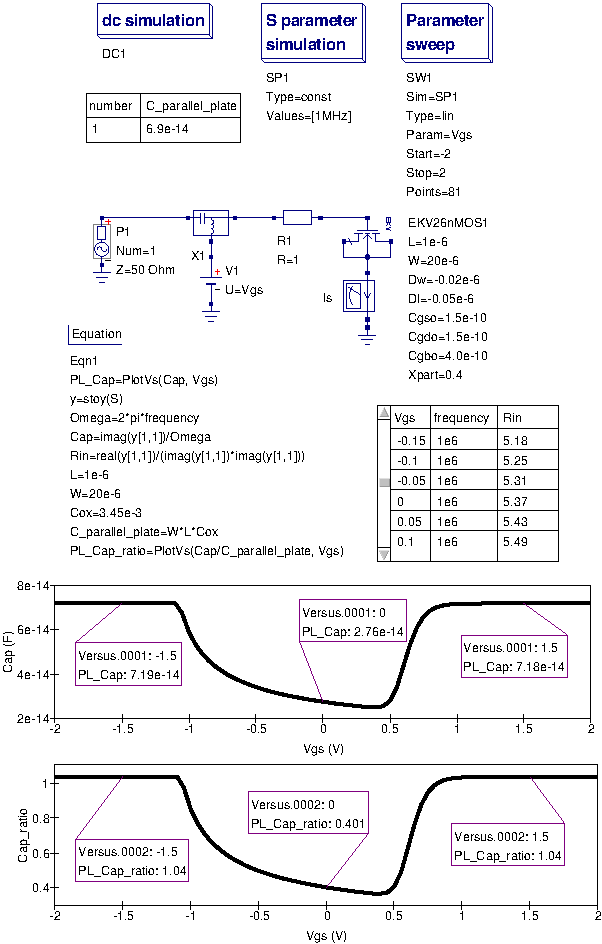
\includegraphics[width=0.8\linewidth]{EKV_fig10}
  \caption{Test circuit for simulating EKV v2.6 charge partitioning effects: Xpart = 0.4 or QD/QS = 40/60}
  \label{fig:EKV10}
\end{figure}  


\tutsubsection{Modelling EKV v2.6 charge partitioning using Qucs EDD}

Complex simulation results like those shown in Fig~\ref{fig:EKV10}
suggest the question ``How do we check the accuracy of the model being
simulated?''. One possible approach is to develop a second model of
the same device based on the same physical principles and equations
but using a different approach like the Qucs EDD/subcircuit modelling
route shown in Fig.~\ref{fig:EKV11}. It is an EDD/subcircuit model of
a long channel EKV v2.6 nMOS device which includes charge
partitioning. Figure~\ref{fig:EKV12} illustrated the same test circuit
as Fig.~\ref{fig:EKV10} and the extracted capacitance and resistance
values for the EDD model of the long channel nMOS device. A number of
features observed from Fig.~\ref{fig:EKV10} and Fig.~\ref{fig:EKV11}
are worth commenting on; firstly that good agreement is recorded
between the two sets of results, secondly that the Verilog-A model
includes both overlap capacitance and drain and gate source
resistances. Hence the slight difference in the capacitance ratio and
the recorded values of Rin above one Ohm for the Verilog-A model.

\begin{figure}
  \centering
  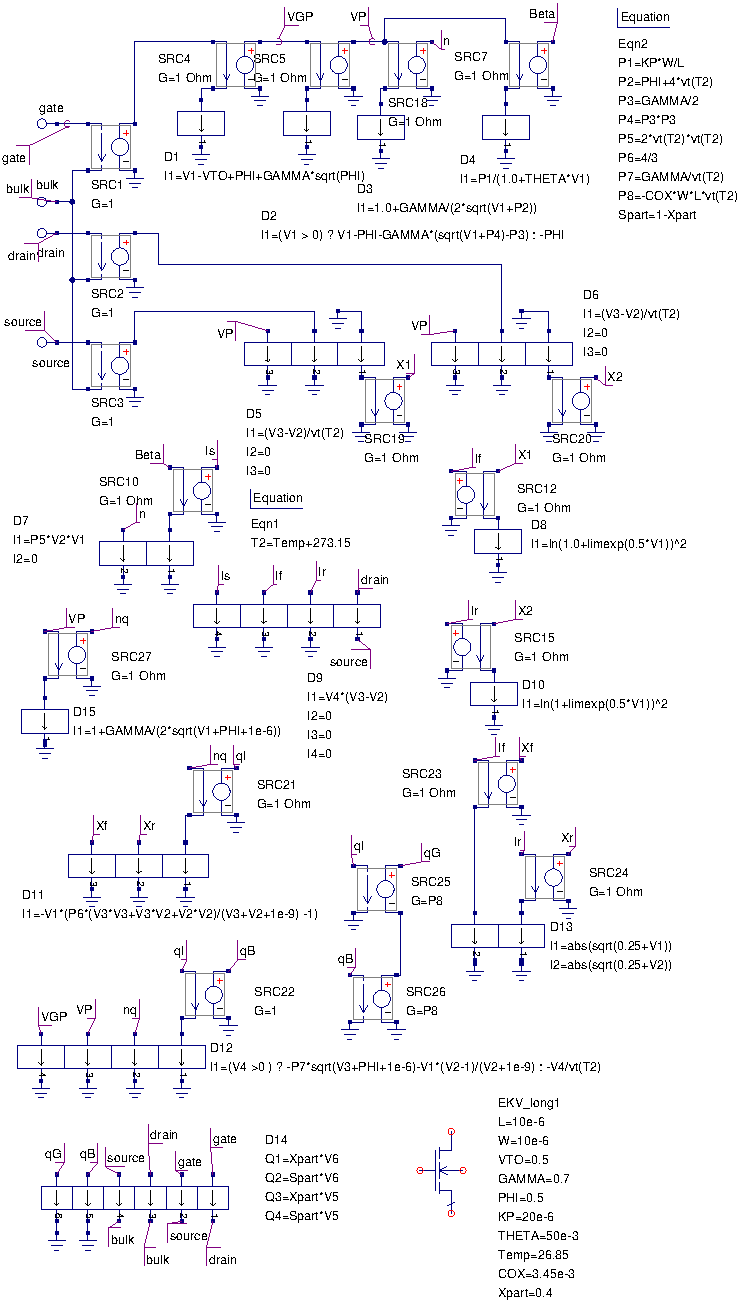
\includegraphics[width=0.6\linewidth]{EKV_fig11}
  \caption{Qucs EDD model for a EKV v2.6 long channel nMOS device with charge partitioning}
  \label{fig:EKV11}
\end{figure}  

\begin{figure}
  \centering
  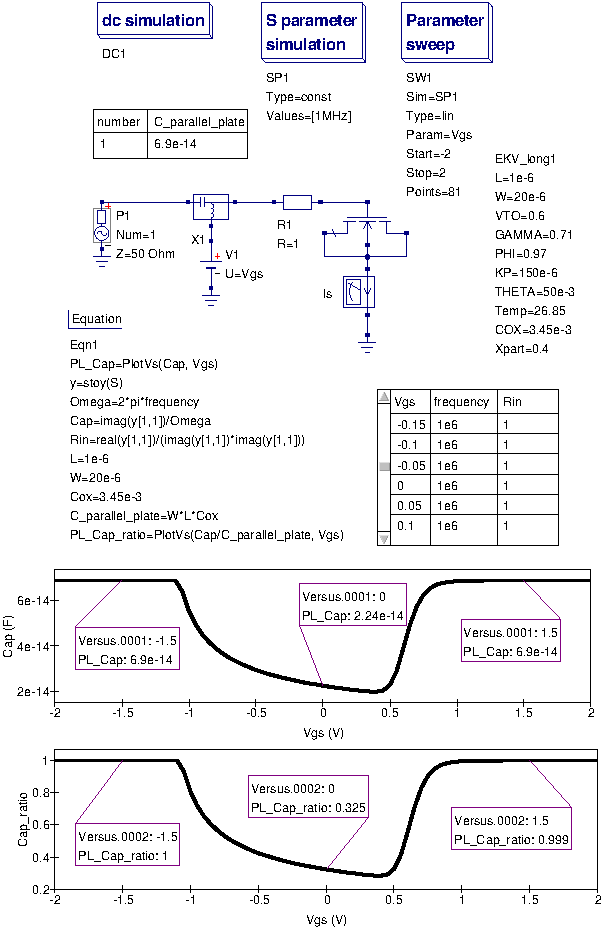
\includegraphics[width=0.8\linewidth]{EKV_fig12}
  \caption{Test circuit for simulating EKV v2.6 EDD model charge partitioning effects: Xpart = 0.4 or QD/QS = 40/60}
  \label{fig:EKV12}
\end{figure}  

\tutsection{End note}

The first update of the Qucs EKV v2.6 model provides users with a more
optimised model, with improved simulation performance and a more
complete charge partitioning scheme.  Even with these changes the
model is still not complete. The nMOS and pMOS Verilog-A code needs to
be unified and a number of optional parameters need to be added to the
Qucs implementation of the EKV v2.6 model.  The next update of the
model is scheduled for the near future, following correction of bug
reports sent in by Qucs users.  Once again my thanks to Stefan Jahn
for all his help and support during the first EKV v2.6 update
development phase.
